\documentclass[a4paper,10pt]{article}
\usepackage[% bw,window,corporate
]{EPFL}
%\def\familydefault{\rmdefault}    % uncomment for serif fonts in body

\title{Graph Networks for Wind Nowcasting}
\subtitle{ Graph Networks offer a flexible way of handling non-regular dataset such as sparse measures in the 3D space. In this work we investigate wether different types of graphs and nodes features can help modelling the wind speed at cruising altitude.}
\author{Arnaud Pannatier}
\narrowmargins                    % uncomment for narrow margins
\symmetricmargins                 % uncomment for equal margins
\unitname{EDIC}{Idiap Research Institute}{Machine Learning Group}
\course{EE-452}{Network Machine Learning}
\usepackage{booktabs}       % professional-quality tables
\usepackage{multirow}
\usepackage{amsmath}
\usepackage{graphicx}
\usepackage{caption}
\usepackage{subcaption}
\usepackage{wrapfig}
\usepackage{placeins}
\usepackage{hyperref}

\newcommand{\ap}[1]{\marginpar{{\tiny \color{red} [AP] #1}}}
\begin{document}

\maketitle

\begin{figure}[htbp]
  \centering
  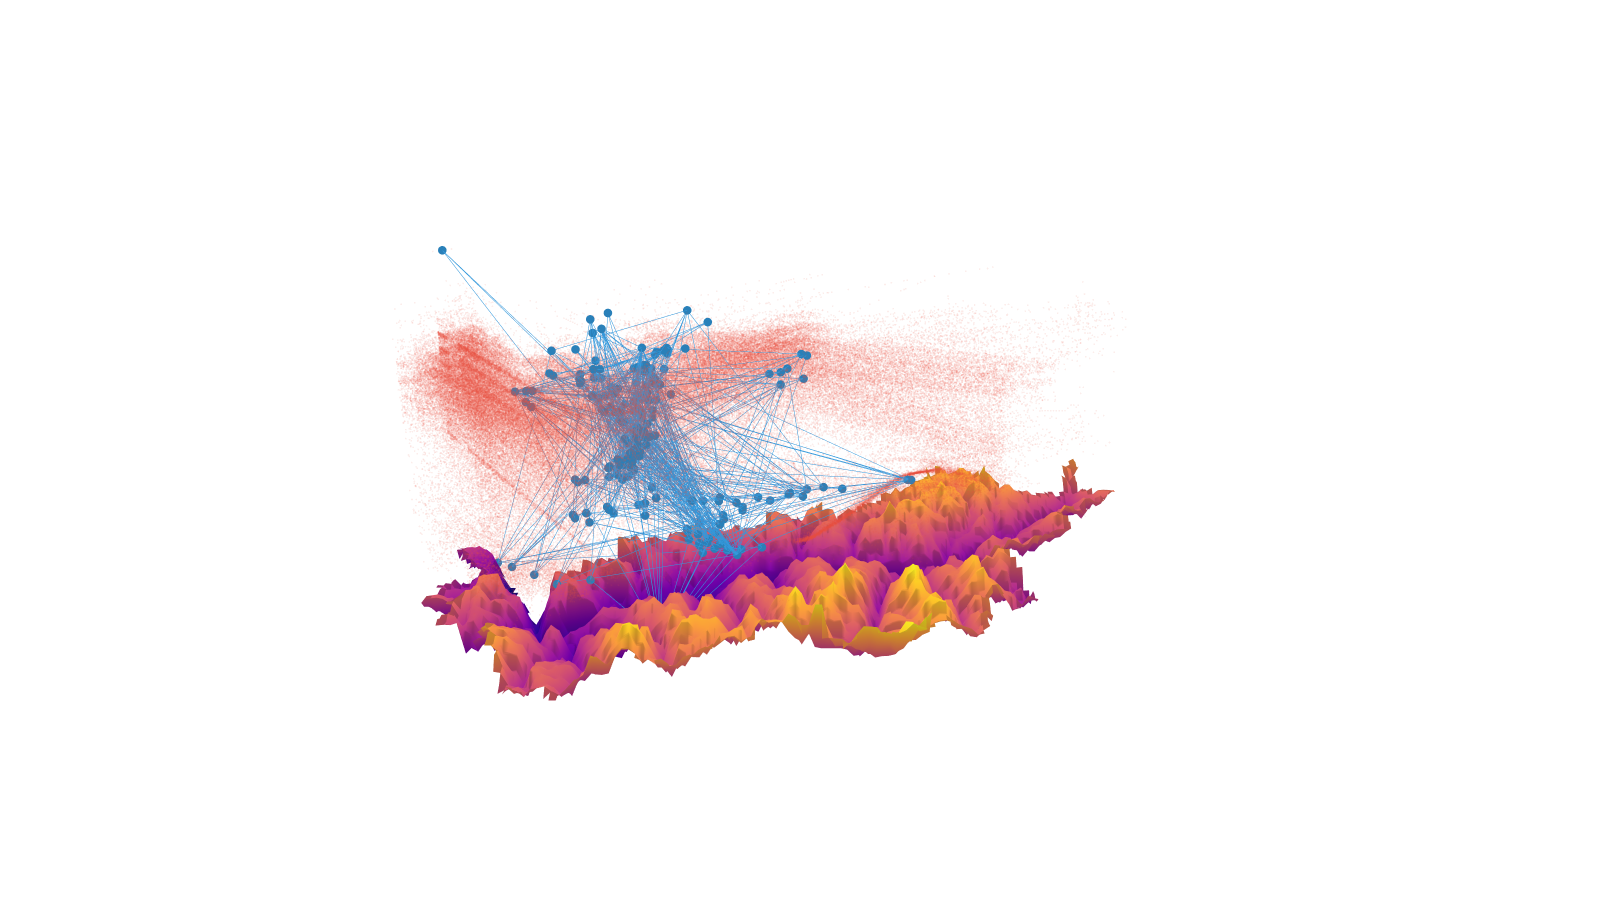
\includegraphics[trim={350 200 450 150},clip,width=\textwidth]{figs/south-gen.png}
\end{figure}

\newpage
\section{Introduction}
Air Traffic Controllers (ATC) need to have access to reliable wind speed forecasts to organize the airspace efficiently. At cruising altitudes, the only measures that one has access to are measured by airplanes that record the wind along their trajectories, and fortunately, as there are a lot of planes flying in the airspace ATCs have recorded a lot of data. Their interest is to be able to a good prediction during the window of time they operate which is rather short (30min up to a few hours) In that range, called nowcasting, one gets the most accurate forecast by extrapolating from the latest measures available rather than trying to solve expensive numerical equations solvers.
It is in that range that deep learning methods can offer a lot, as meteorological data is often highly available. Sadly this data are recorded along trajectories and is sparse in space, so we cannot uses standard methods such as CNN to deal with it. We noticed that it could be a good candidate for Graph Networks are their inductive bias makes them good candidates for this task.

This work will use graph networks to forecast the wind speed at cruising altitudes. We will use the \textit{SkySoft ATM MALAT Wind Speed Dataset} \cite{skysoft2021dataset} and starting from an Graph Element Network (GEN) \cite{alet2019gen} implementation, we will analyse the effect of the topology of the graphs and different nodes and edge features on the performance of the model. The implementation of the different models is publicly available \footnote{The code of this work is available at \url{https://github.com/ArnaudPannatier/nml-project}}


\subsection{Problem formulation}

Let $\mathbb{X}, \mathbb{I}, \mathbb{O}$ be three bounded metric spaces, and define two functions $f : \mathbb{X}\rightarrow \mathbb{I}$, mapping from data to the input space, and $g : \mathbb{X}\rightarrow \mathbb{O}$ mapping to the output space.
In the case of wind nowcasting, $\mathbb{X} = \mathbb{R}^{3} \times \mathbb{R}^{+}$, which corresponds to 3 spatial coordinates and one temporal and $\mathbb{I} = \mathbb{O} = \mathbb{R}^{2}$ which encode the wind in the $(x,y)$ plane.
We want to learn the transformation which maps a function $f$ to $g$.
We only have access to $f$ by data $(x, i)  \in \mathbb{X} \times \mathbb{I}$ of measures $i$ at position $x$ and we know $g$ only through a set $(x', o) \in \mathbb{X} \times \mathbb{O}$ of measurements $o$ at position $x'$.
So we learn this mapping from data using multiple sets of meaures corresponding to many $(f,g)$ pairs with the objective of minimizing the distance in the output metric space $\mathbb{O}$ between predictions and references.

\section{Related works}

\subsection{Graph Element Networks (GENs)} \label{ssec:gen}
Graph Element Networks \cite{alet2019gen} aim to model field transformations using a non-regular graphs with nodes in the underlying space $\mathbb{X}$. Each measurement $(x, i)$ is encoded using a small MLP, the initial latent feature of one node is then computing by averaging the embeddings of the measurements based on their distance to the node. The model then process this latent variable using $T \in \mathbb{N}$ steps of message passing, using the following equations:

\begin{align}
  m_{ij}^{t + 1} = m_e(l_{i}^{t}, l_{j}^{t}) \\
  l_{j}^{t + 1} = m_{n}(l_{i}^{t}, \sum_{(i,j) \in \mathcal{N}} m_{ij}^{t + 1})
\end{align}

Where $m_e, m_n$ are multilayer perceptrons and $l_{i}^{t}$ is the latent state of nodes $i$ at the $t$-th step of message passing. In that representation, no edge features are used.
To predict a value at a new query position, the model linearly extrapolates in latent space and decodes using a small MLP modeling the transformation from latent to output space.

\begin{figure}[htbp]
  \centering
  \includegraphics[width=\textwidth]{figs/GEN}
  \caption{GEN architecture \cite{alet2019gen}. The measures are first encoded to a latent space, then the initial node feature is computed by aggregating the closer encoded measures, the processing is done by message passing and the final measures are retrieved by first interpolating the features of the nodes at the query position and then decoding.}
\end{figure}

\ap{advantages -- drawbacks}

\subsection{Finite Element Networks}

Traditional PDEs solvers model the domain using regular grids, but this has some drawbacks as some parts of the space might be more complicated to model than the others. One way of dealing with this problem is to use a Finite Element method approach \cite{hughes2012finite}, which uses a non-regular graph that can be denser in the more complex regions and coarser in the smoother regions.

\ap{advantages --drawbacks}


\section{Exploration}
\subsection{Graph Types}

Usually, the mesh for FEM simulations is created beforehand with denser regions where we expect the field to behave more complicatedly way. Meshes for this simulation are usually a triangulation of the region of interest. The triangulation subdivides the space into nonoverlapping triangles, such that each triangle have either a side or a vertex in common or is disjoint. A density parameter defines the finesse of the triangulation. The graph generated by this triangulation scheme is such that there is an edge between two nodes only if there are close in the Euclidean sense. The degree distribution of these graphs has only small values corresponding to the local neighborhood.

\begin{wrapfigure}{l}{0.3\textwidth}
  \centering
  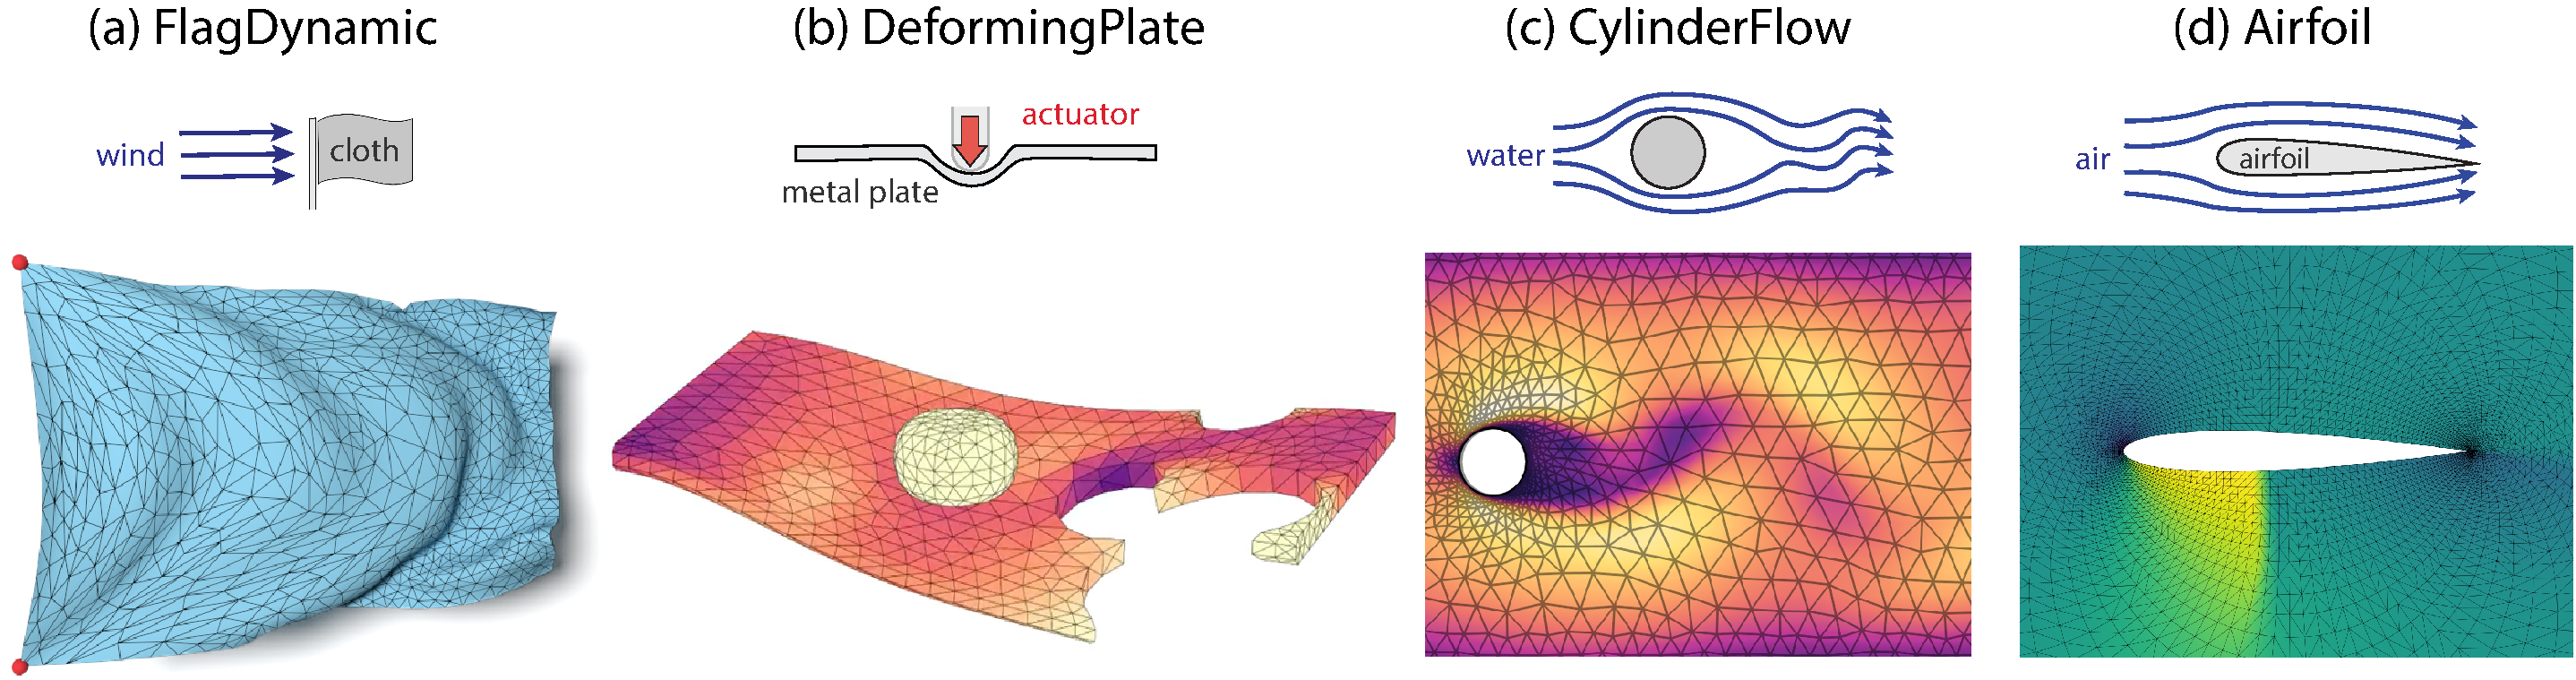
\includegraphics[trim={780 0 300 50},clip,width=0.3\textwidth]{figs/mesh-dataset}
  \caption{Typical FEM meshing \cite{pfaff2020learning}}
\end{wrapfigure}

For GENs, the original way of creating graphs is to create a grid mesh that covers the whole space, and encode the node position as parameters of the model, so that it can be optimized by gradient descent during training. In that case, the graph structure remains similar to the initial grid structure.

In both apporaches, only those graph structures have been used. In this work, we will consider three approaches for our graph topology. The first one, considered as a baseline is constructed as follows: First, we will take the $k$-means of the measurement positions and we will add edges between the nearest neighbors. The second one will be a random network where the nodes' position and their edges are taken at random, we will try different parameters $p$ and analyze their effect on the quality of the model.

For the last graph structure, we will use a Barab\'asi-Albert model scheme for growing a graph to a given number of nodes, we will then associate to each node one of the $k$-means positions. FEM and GEN are traditionally only using edges between neighbors, but we think that having long-range connections and hubs can help the models to process the information more efficiently. A sketch of the graphs can be found in Figure \ref{fig:graphs}.


\subsection{Features}

In this work, we will focus on nodes and edges features as we are using the graph network to do regression over the whole space. We won't need to aggregate the features over the whole graph.


\subsection{Nodes features}
As described in section~\ref{ssec:gen}, GEN is only using node features that are computed by aggregating the learned embeddings of the measures based on their distance. We will visualize their value in some very unbalanced cases and the effect of the message passing on the features. This will help us to choose the message passing steps and guide us through the analysis of the different graph structures.

We assume that this part is the most important to get a good model. So we will explore different strategies and measure their impact on the model. First, we will try to use no encoder and aggregate the normalized measured values. With this approach, we delegate the whole processing to the graph networks, and we think this should be already a strong baseline as the outputs values are strongly related to these initial values. We will then try to use fixed sine-cosine positional encodings ~\cite{vaswani2017attention} and 3D positional fixed sine-cosine positional encodings ~\cite{chu2021conditional}. The idea is to use a simple $1d$ positional encoding that takes as input the position $x,y$ or $z$ and maps into a feature space of larger dimensionality. These encodings can be added or concatenated and we will try both approaches to see which one helps during training. A sketch of these positional encodings can be found in Figure \ref{fig:posenc}

\begin{figure}
  \begin{subfigure}{0.4\textwidth}
    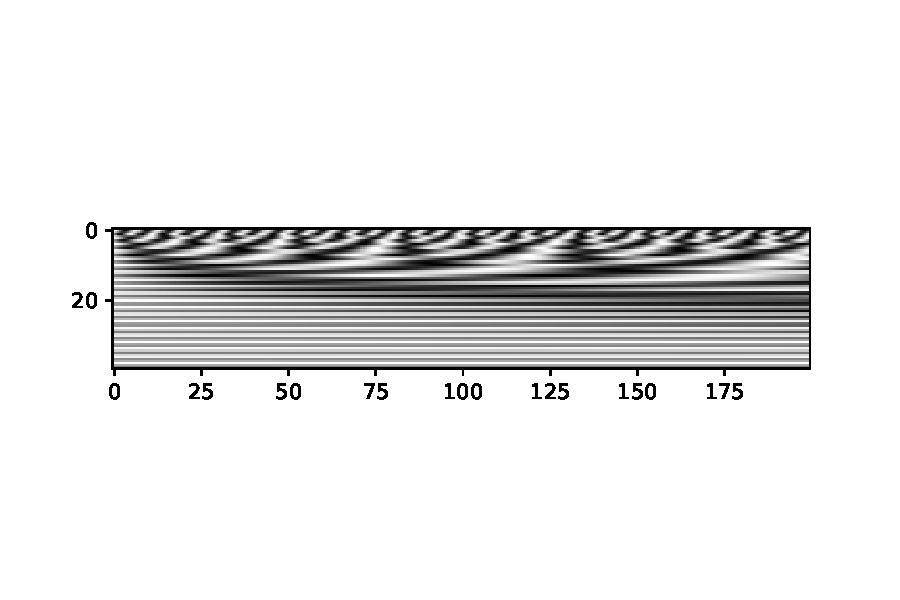
\includegraphics[width=\textwidth]{../windgraph/1dposenc}
  \end{subfigure}
  \begin{subfigure}{0.5\textwidth}
    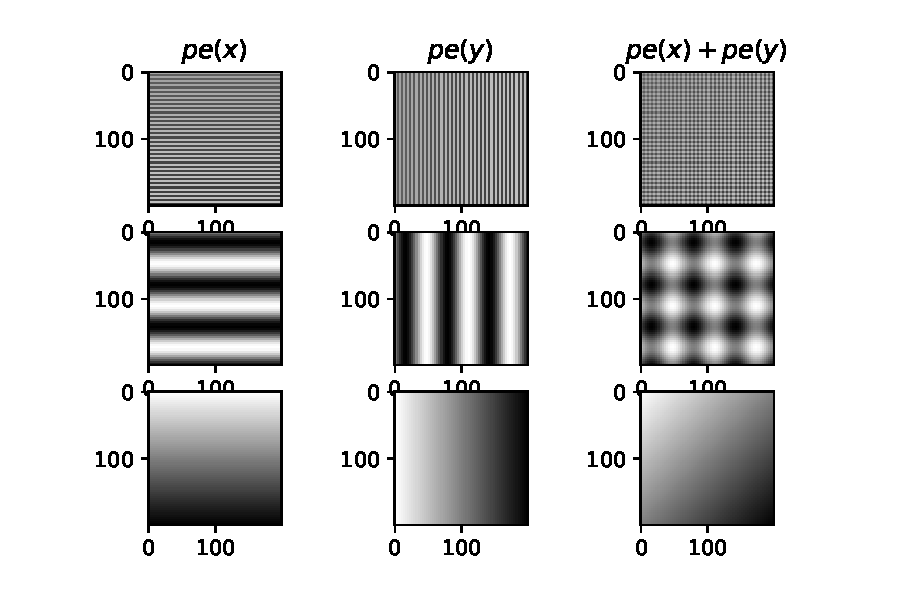
\includegraphics[width=\textwidth]{../windgraph/posenc}
  \end{subfigure}
  \caption{Generalization of 1d positional encoding (right) to 2d/3d with the choice of concatenating (first two columns) or adding (last columns.)}
  \label{fig:posenc}
\end{figure}

\subsection{Edge features}
A contribution of this work is to add edge features to GENs. We think that good graph networks for space modeling should be able to compute an approximation of the derivatives of values in the graph. We will take Euler scheme as an inspiration and have an explicit design for edge features that allows this kind of computation. We will make an ablation with learned features and see their effect on the quality of the model.

The inspiration is that the evolution of the wind speed is governed by the local movement equation:
\begin{equation}
  \rho \mathbf{g} - \nabla p = \rho\frac{d\mathbf{v}}{dt}
\end{equation}

Roughly when using a traditional solver we will approximate the spatial and temporal derivatives using finite differences:
\begin{equation}
  \frac{u_{i}^{n + 1} - u_i^{n}}{\Delta t} = F_{i}^{n}(u,x,t, \frac{\partial u}{\partial x}, i\frac{\partial^2 u}{\partial x^{2}}    )
\end{equation}
So we think that adding edge features that hold the distance between two nodes can help model the PDEs.


\section{Exploitation}

\subsection{Graph Types}

The four different graphs that we tried are depicted in Figure \ref{fig:graphs}. The first-row show the case where the nodes are fixed during training and the second row contains graphs were the node position is optimized during training with gradient descent.
The performance of the different graph types is displayed in Table \ref{tab:graphs}. We ran experiments using ten different seeds, for each node embedding and the position of the graph could be optimized in the case where the structure is fixed.
We see that allowing positions to move during training (\textsc{Adapt} in the table) are always performing better than their fixed counterpart. Random Graphs are the baseline and we expect them to perform poorly as they are initialized randomly without taking into account additional insight that we can have about the dataset. We see that indeed their performance is worse than the other models, but when the position of the nodes can be optimized Random Networks are on par with the best network structure.

Traditional approaches are using only edges between neighbors we think that they thought that for modeling the dynamics of the wind the information should only influence its neighborhood. However, we found that the best performing graphs (Random Networks with optimized position and Barabasi-Albert graphs) achieve the best performance. This might be due to the presence of hubs and long-range interaction which might helps the models to organize the information hierarchically.


\begin{figure}[htbp]
  \begin{subfigure}{0.24\textwidth}
    \centering
    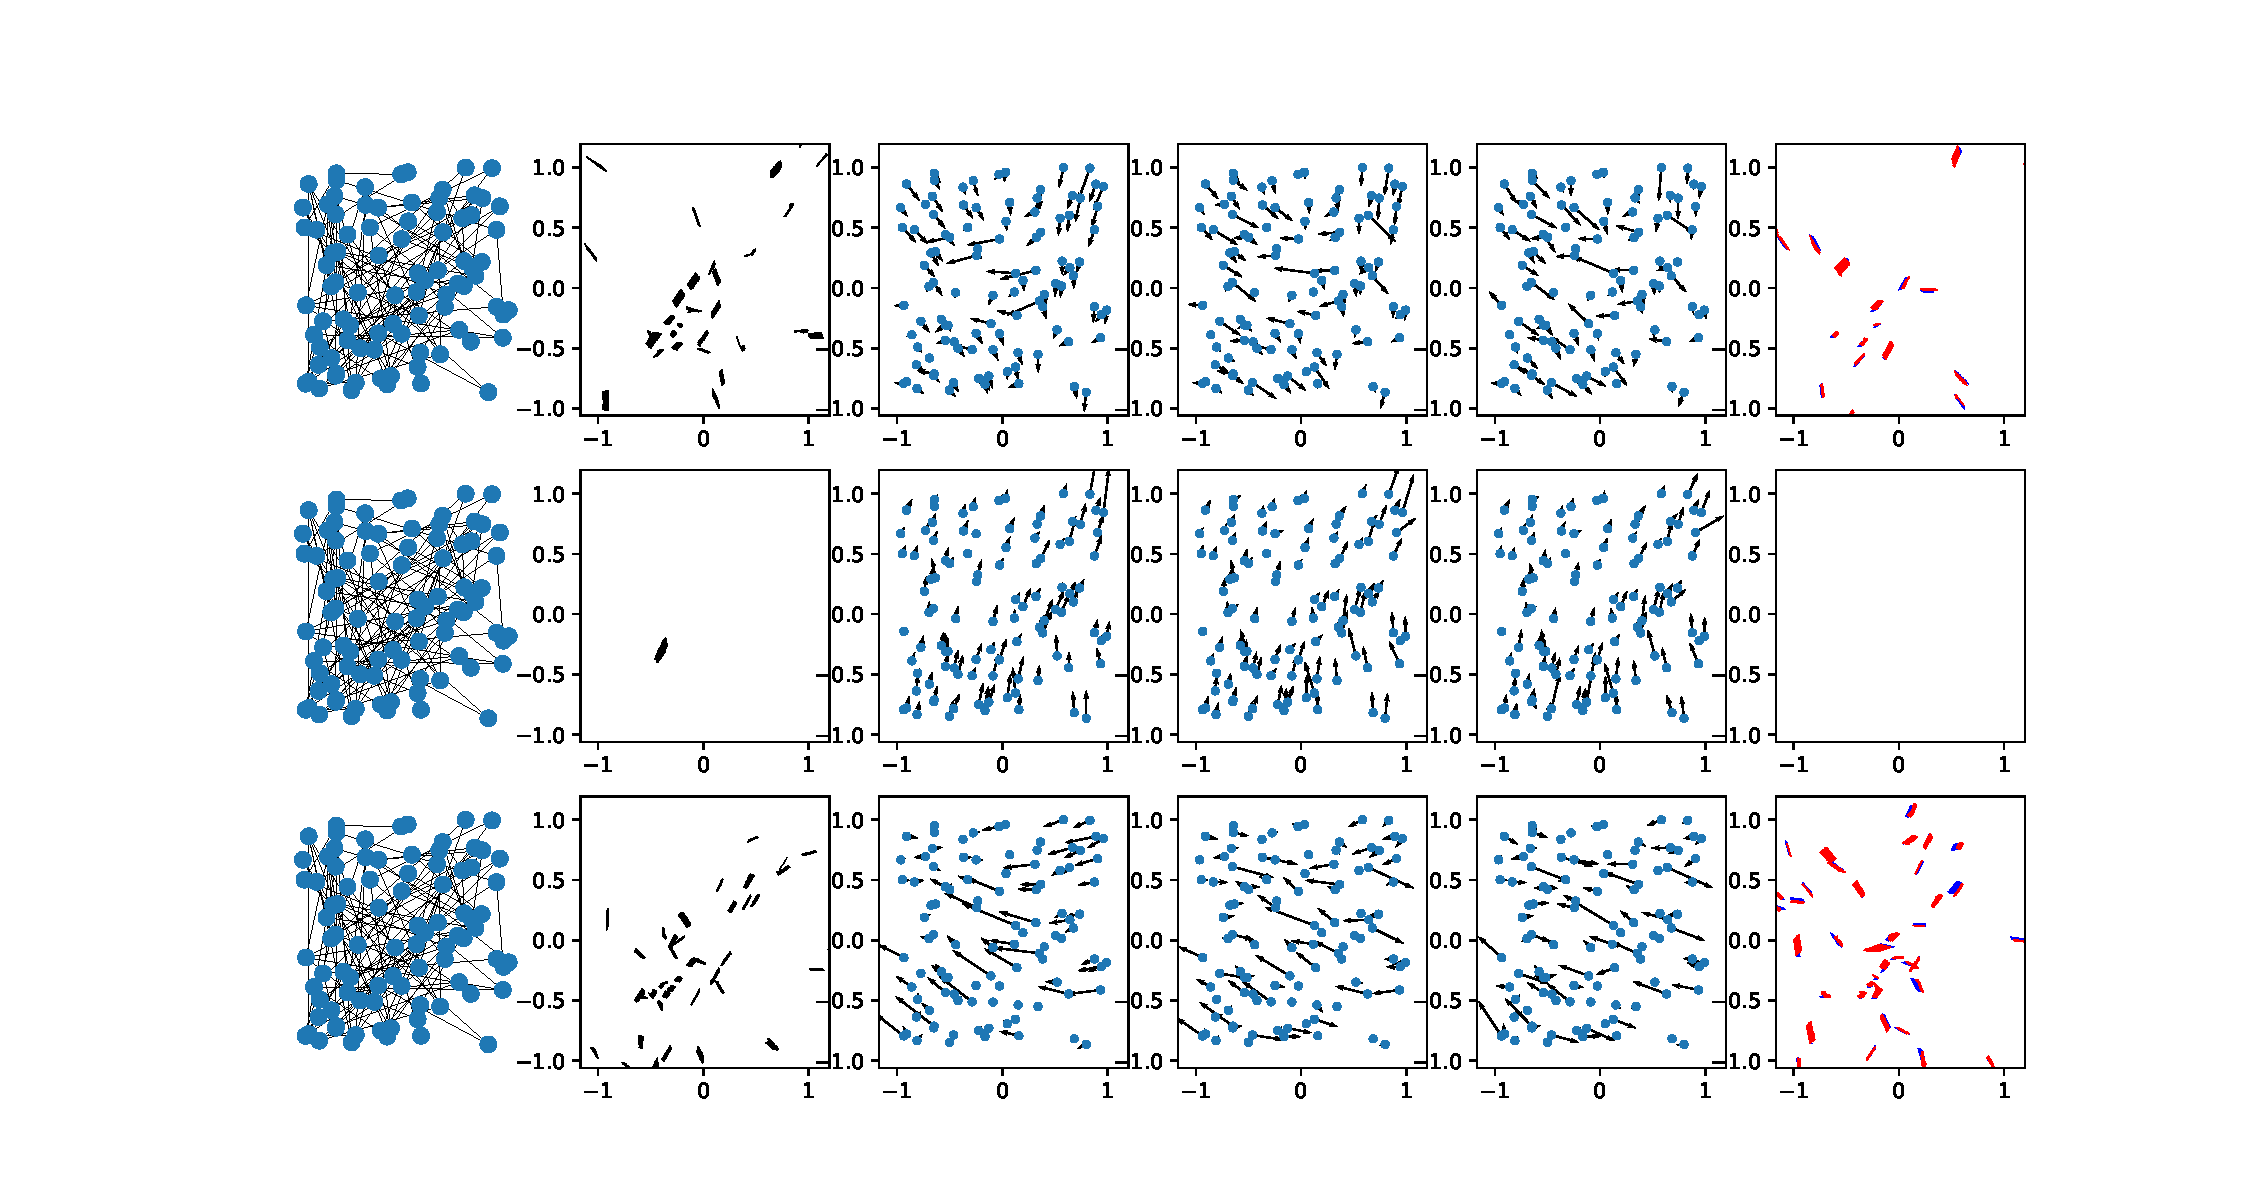
\includegraphics[trim={0 13.2cm 29.35cm 0},clip,width=\textwidth]{../results/pdfs/rn1-100N-noemb-fixed}
    \caption{Random network with $p=1\%$}
  \end{subfigure}
  \begin{subfigure}{0.24\textwidth}
    \centering
    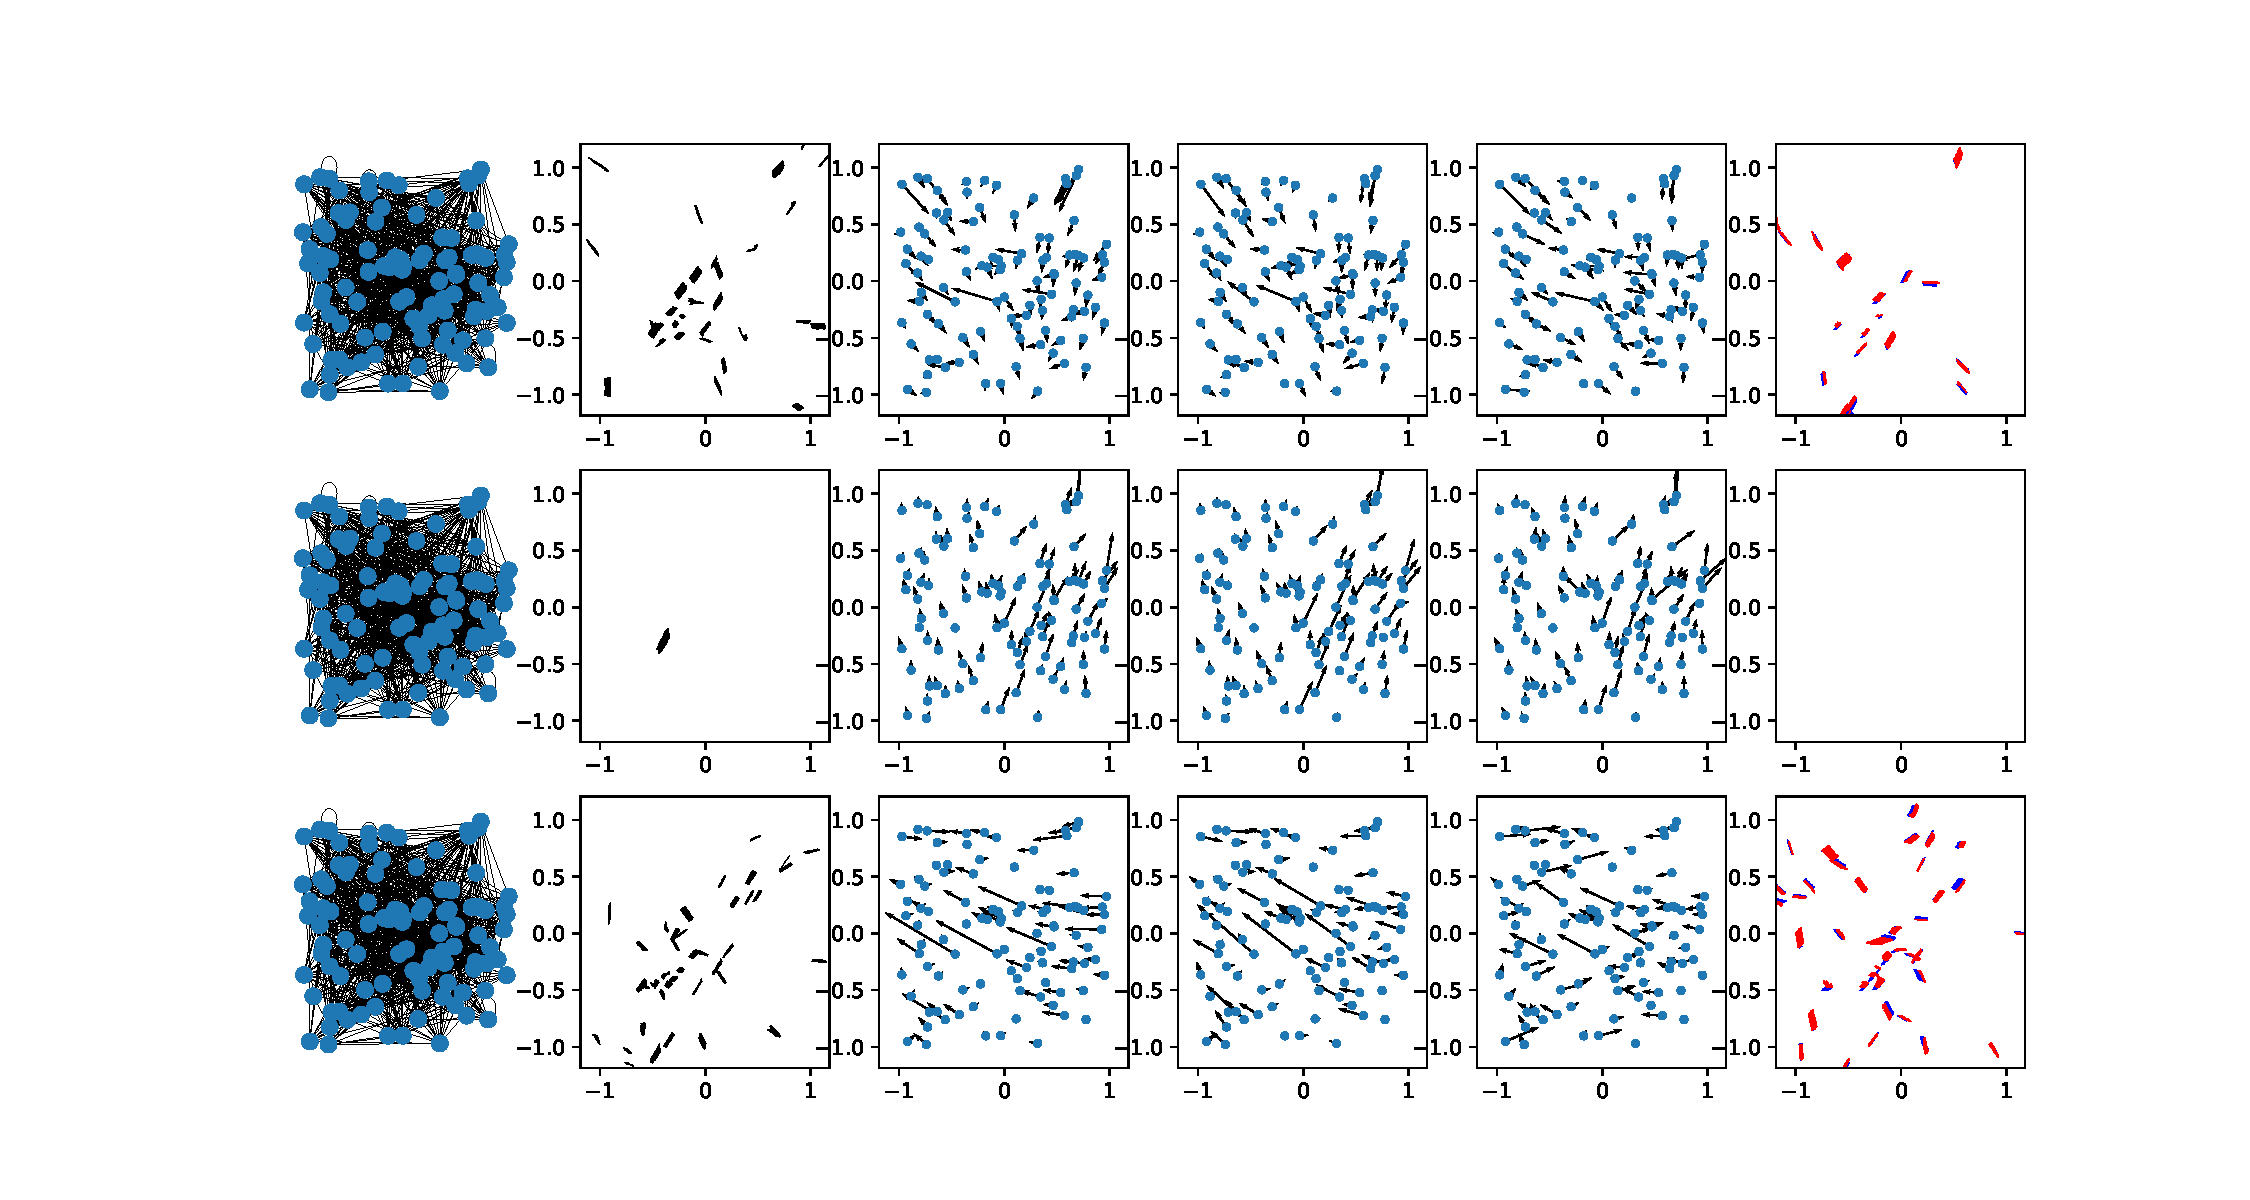
\includegraphics[trim={0 13.2cm 29.35cm 0},clip,width=\textwidth]{../results/pdfs/rn10-100N-noemb-fixed}
    \caption{Random network with $p=10\%$}
  \end{subfigure}
  \begin{subfigure}{0.24\textwidth}
    \centering
    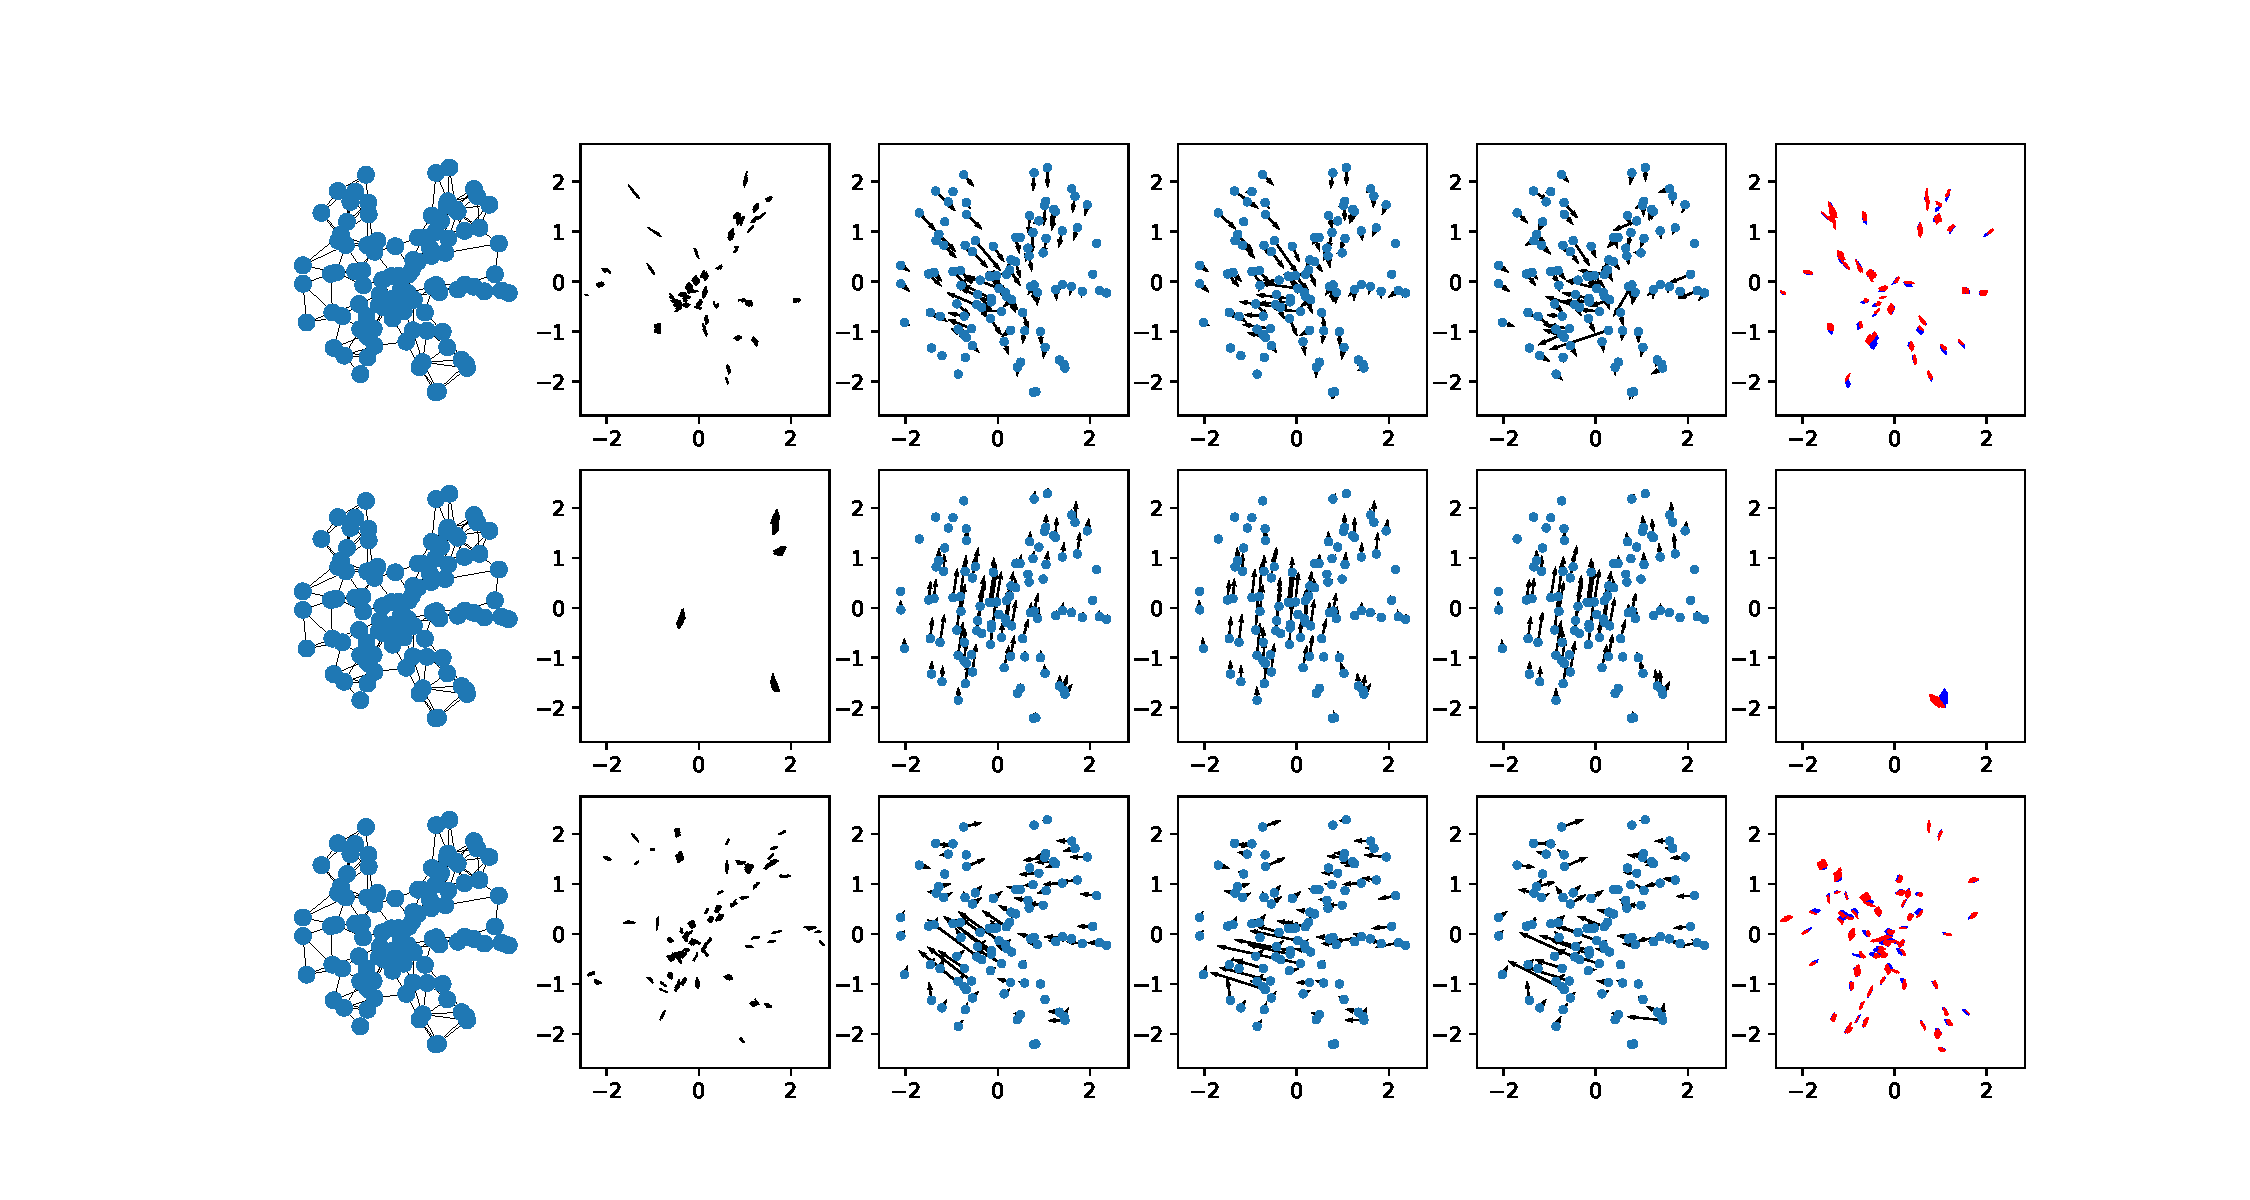
\includegraphics[trim={0 13.2cm 29.35cm 0},clip,width=\textwidth]{../results/pdfs/nn-100N-noemb-fixed}
    \caption{$k$-means, 3nn}
  \end{subfigure}
  \begin{subfigure}{0.24\textwidth}
    \centering
    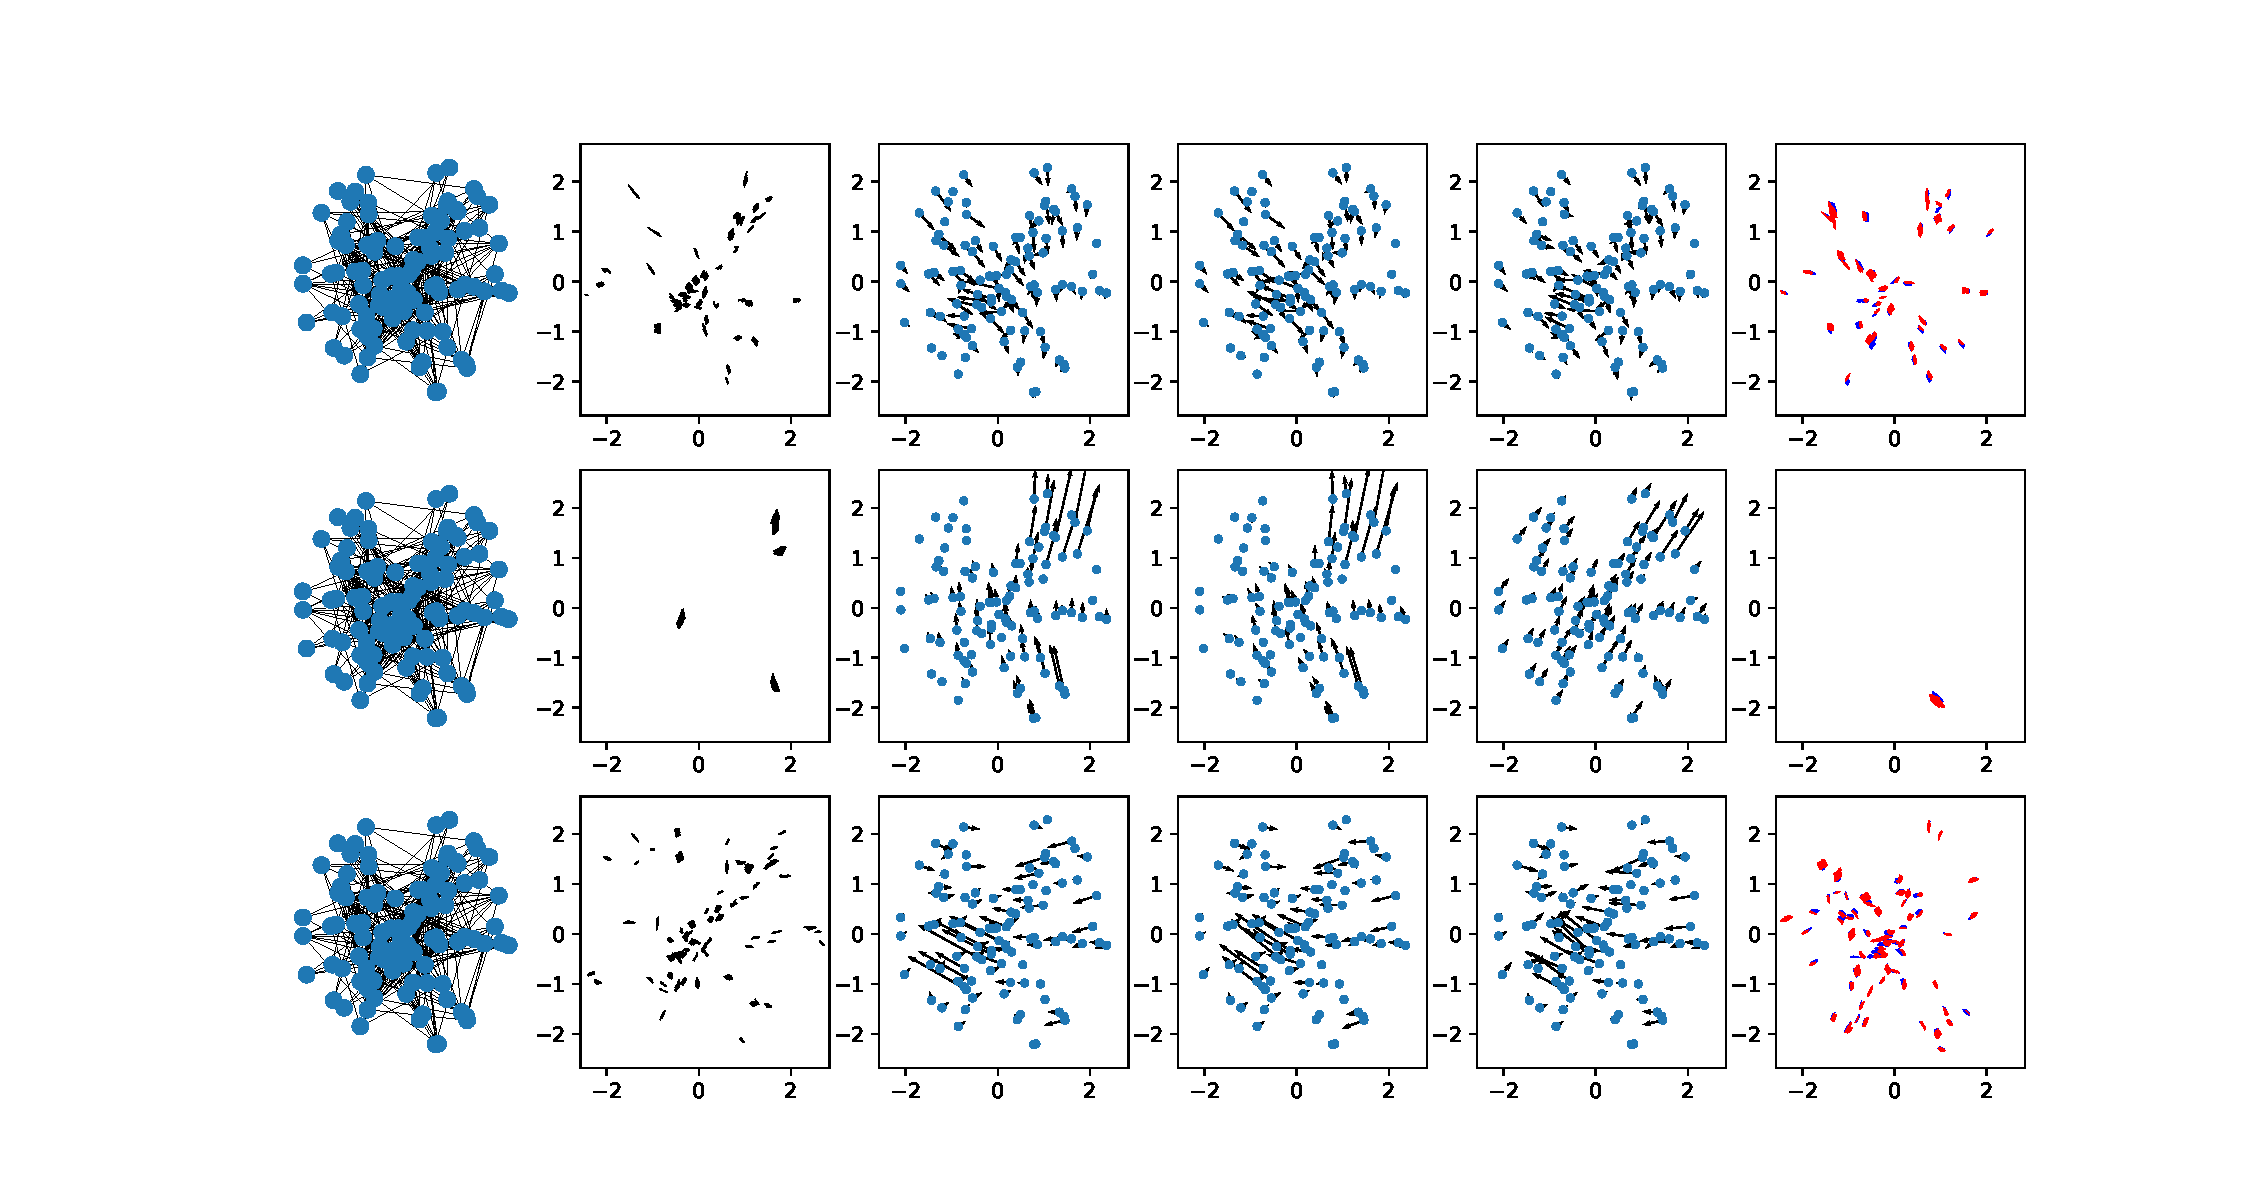
\includegraphics[trim={0 13.2cm 29cm 0},clip,width=\textwidth]{../results/pdfs/ba-100N-noemb-fixed}
    \caption{$k$-means, BA}
  \end{subfigure}
  \begin{subfigure}{0.24\textwidth}
    \centering
    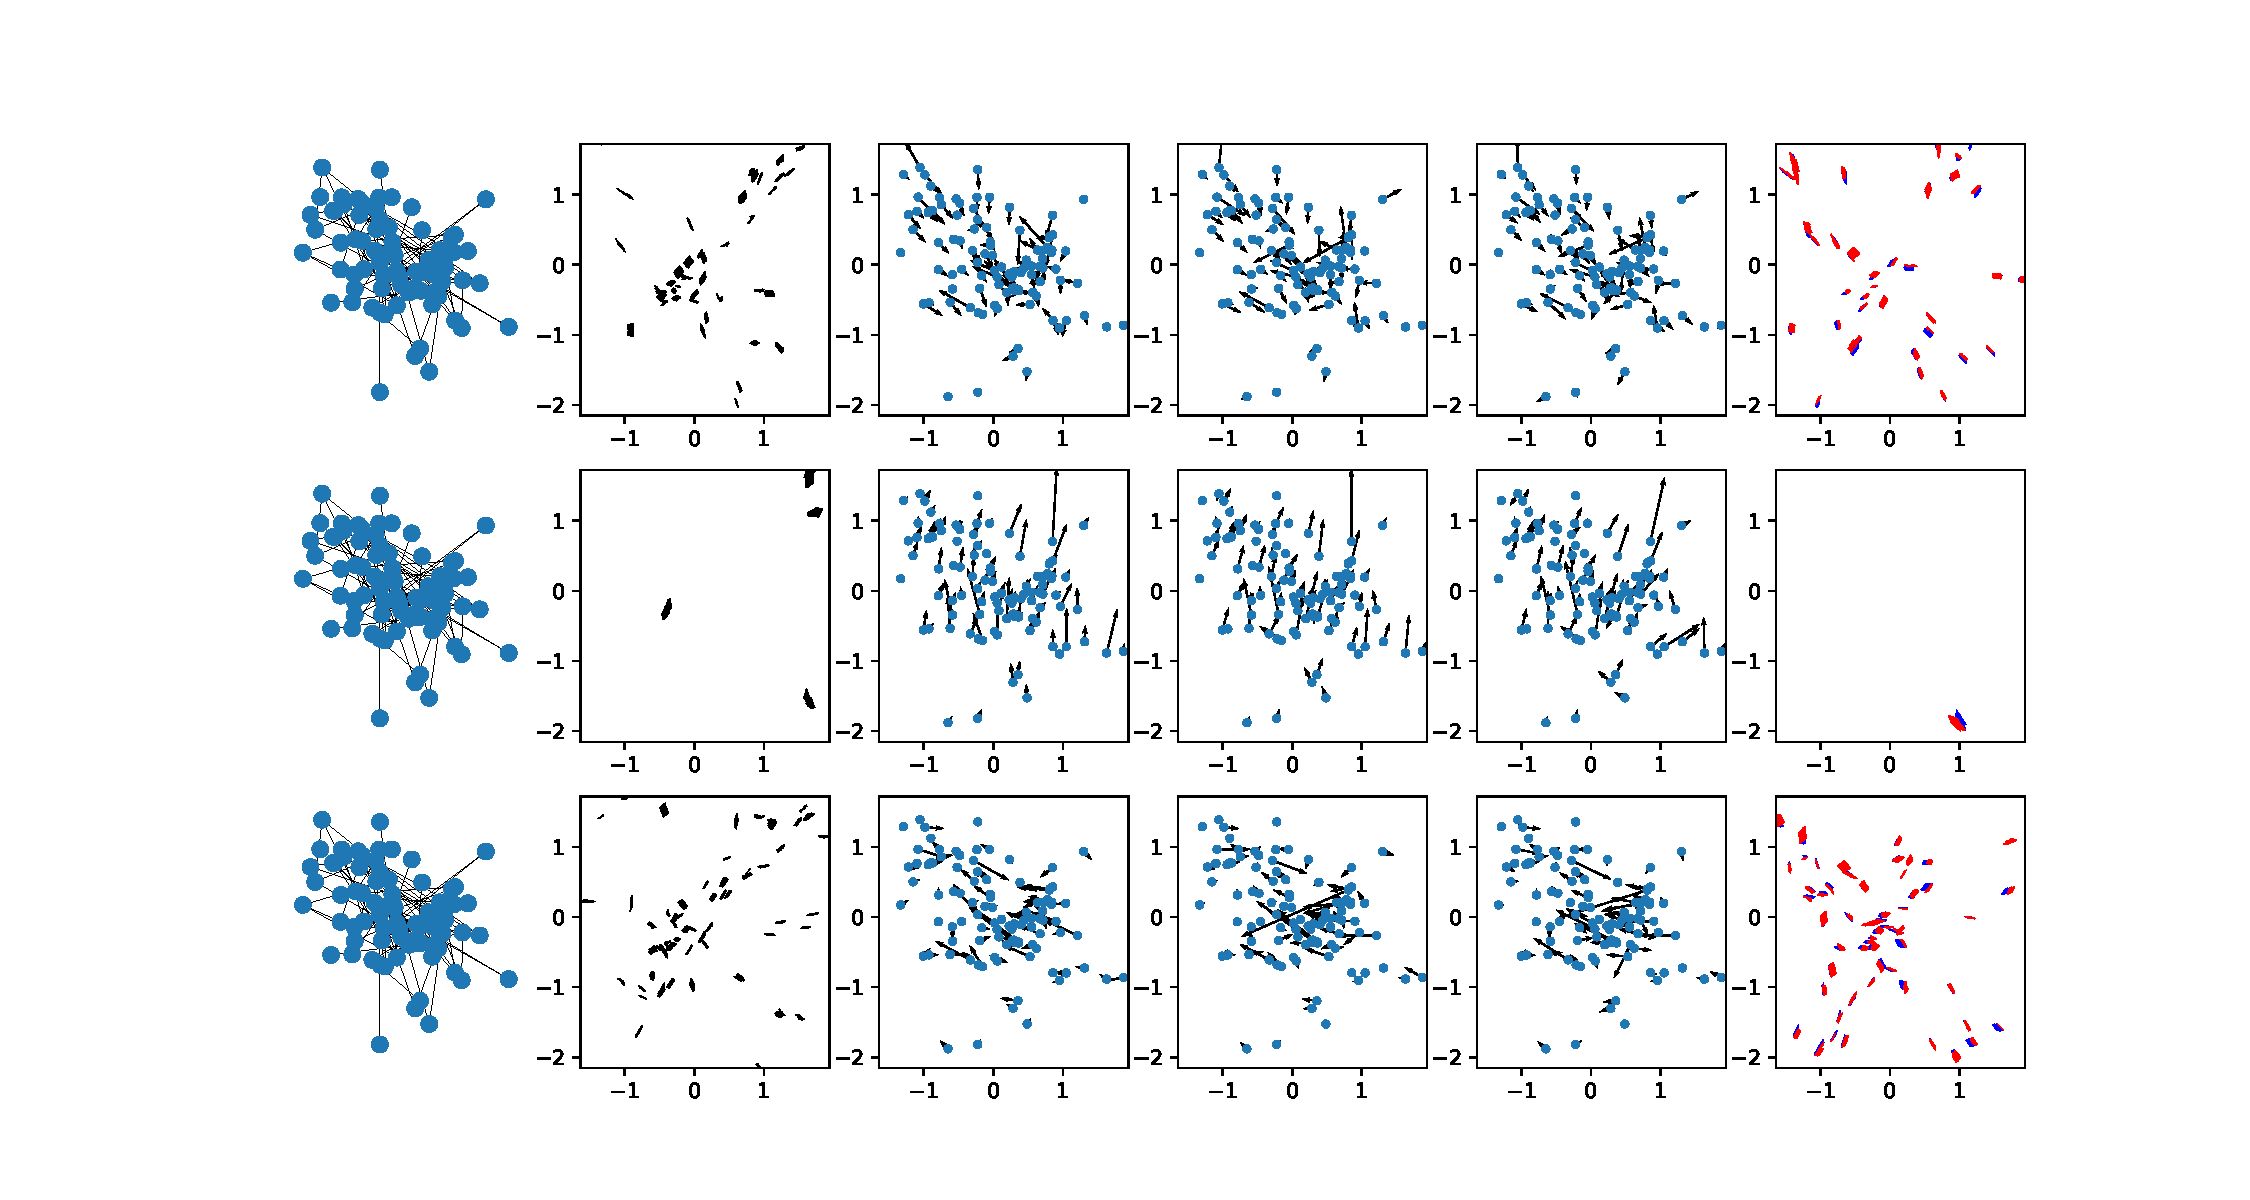
\includegraphics[trim={0 13.2cm 29cm 0},clip,width=\textwidth]{../results/pdfs/rn1-100N-noemb0}
    \caption{Random network with $p=1\%$}
  \end{subfigure}
  \begin{subfigure}{0.24\textwidth}
    \centering
    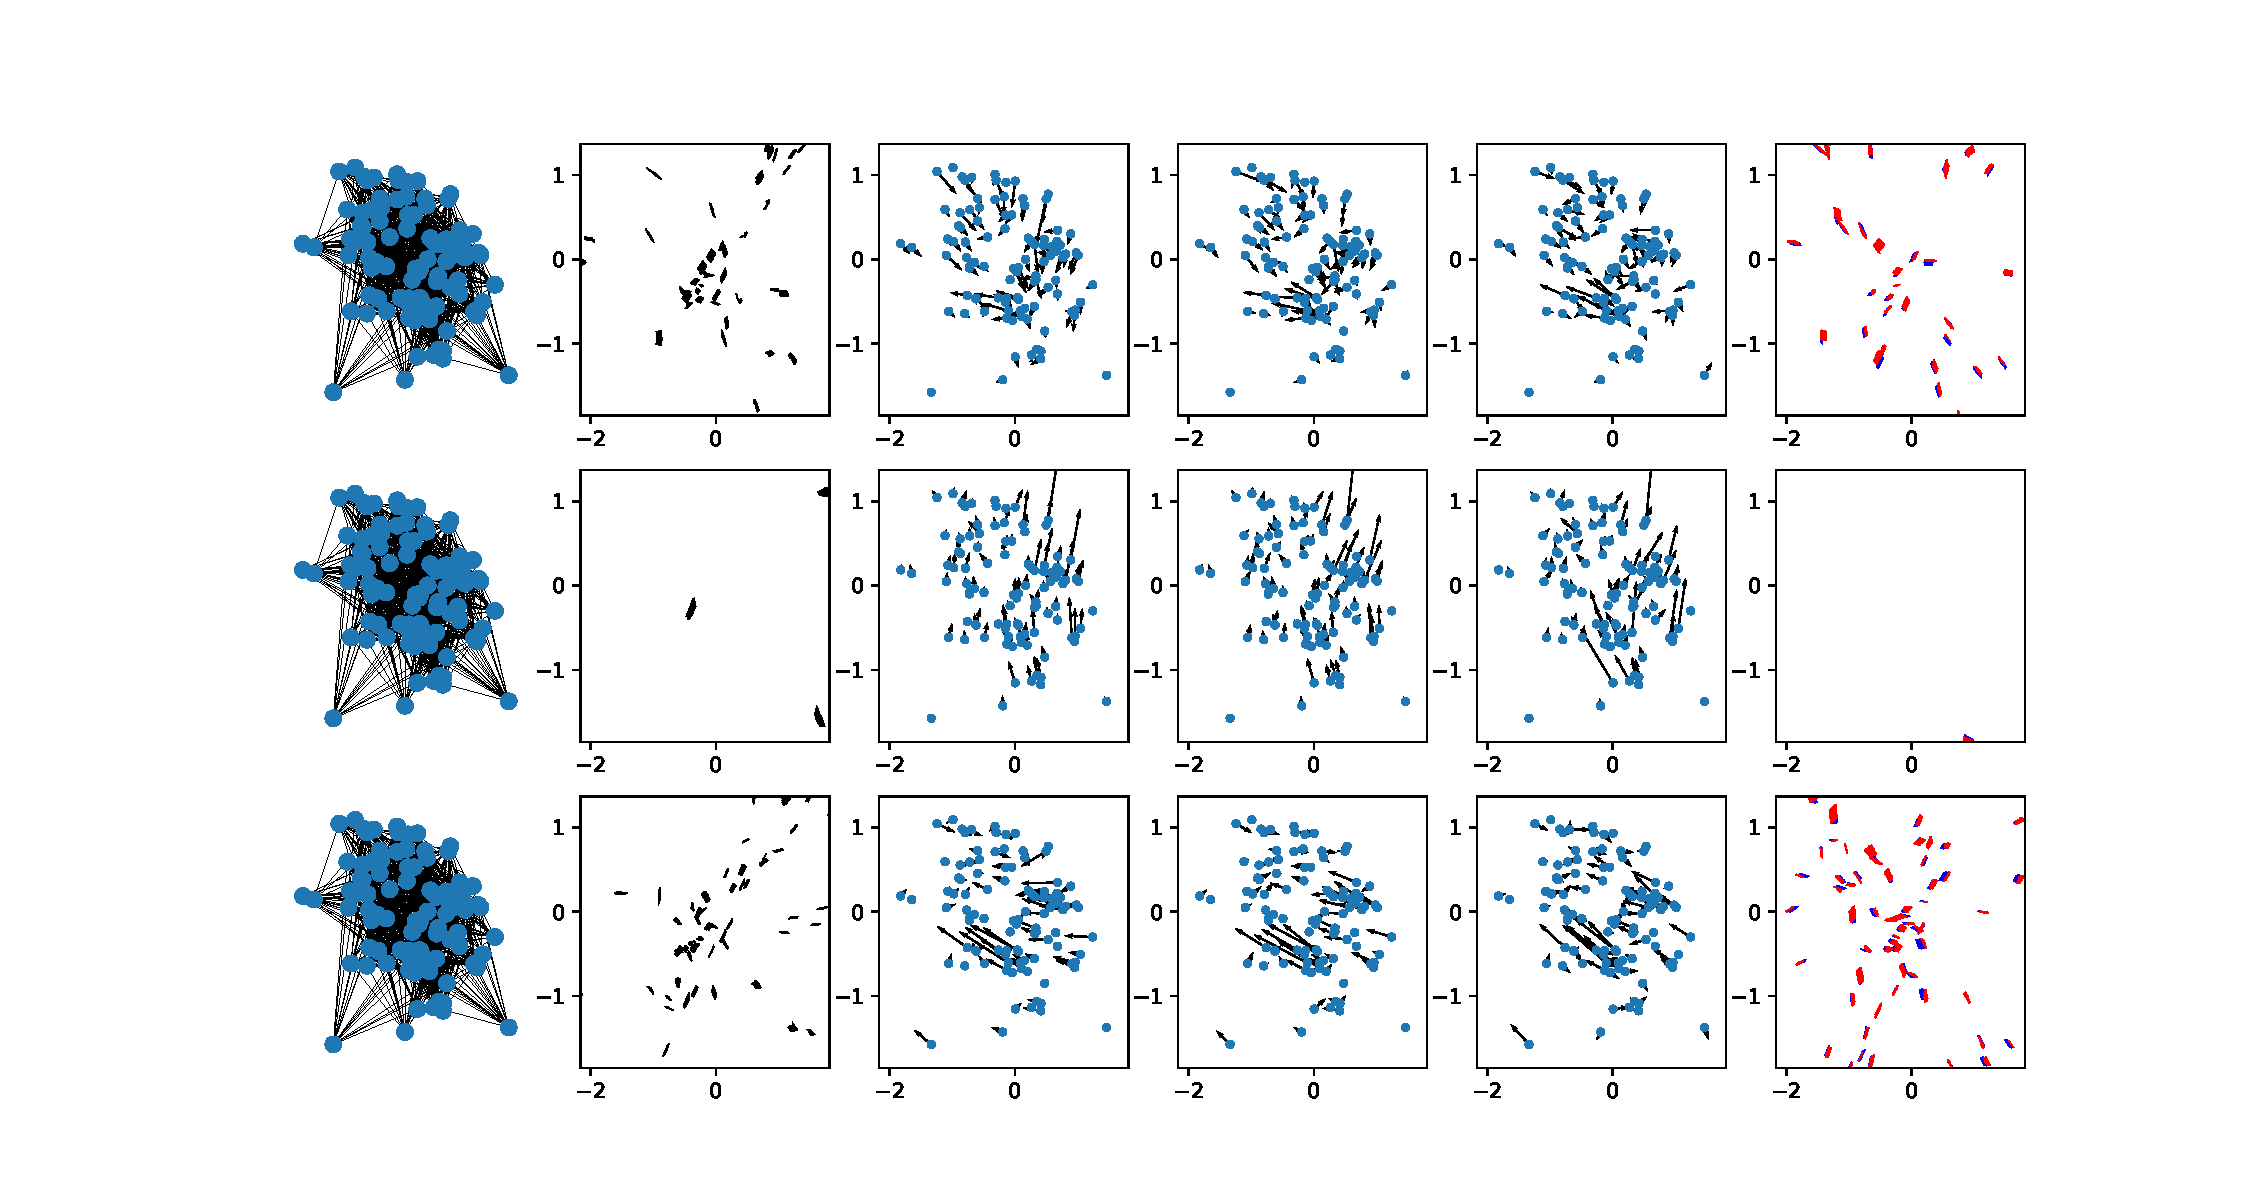
\includegraphics[trim={0 13.2cm 29cm 0},clip,width=\textwidth]{../results/pdfs/rn10-100N-noemb0}
    \caption{Random network with $p=10\%$}
  \end{subfigure}
  \begin{subfigure}{0.24\textwidth}
    \centering
    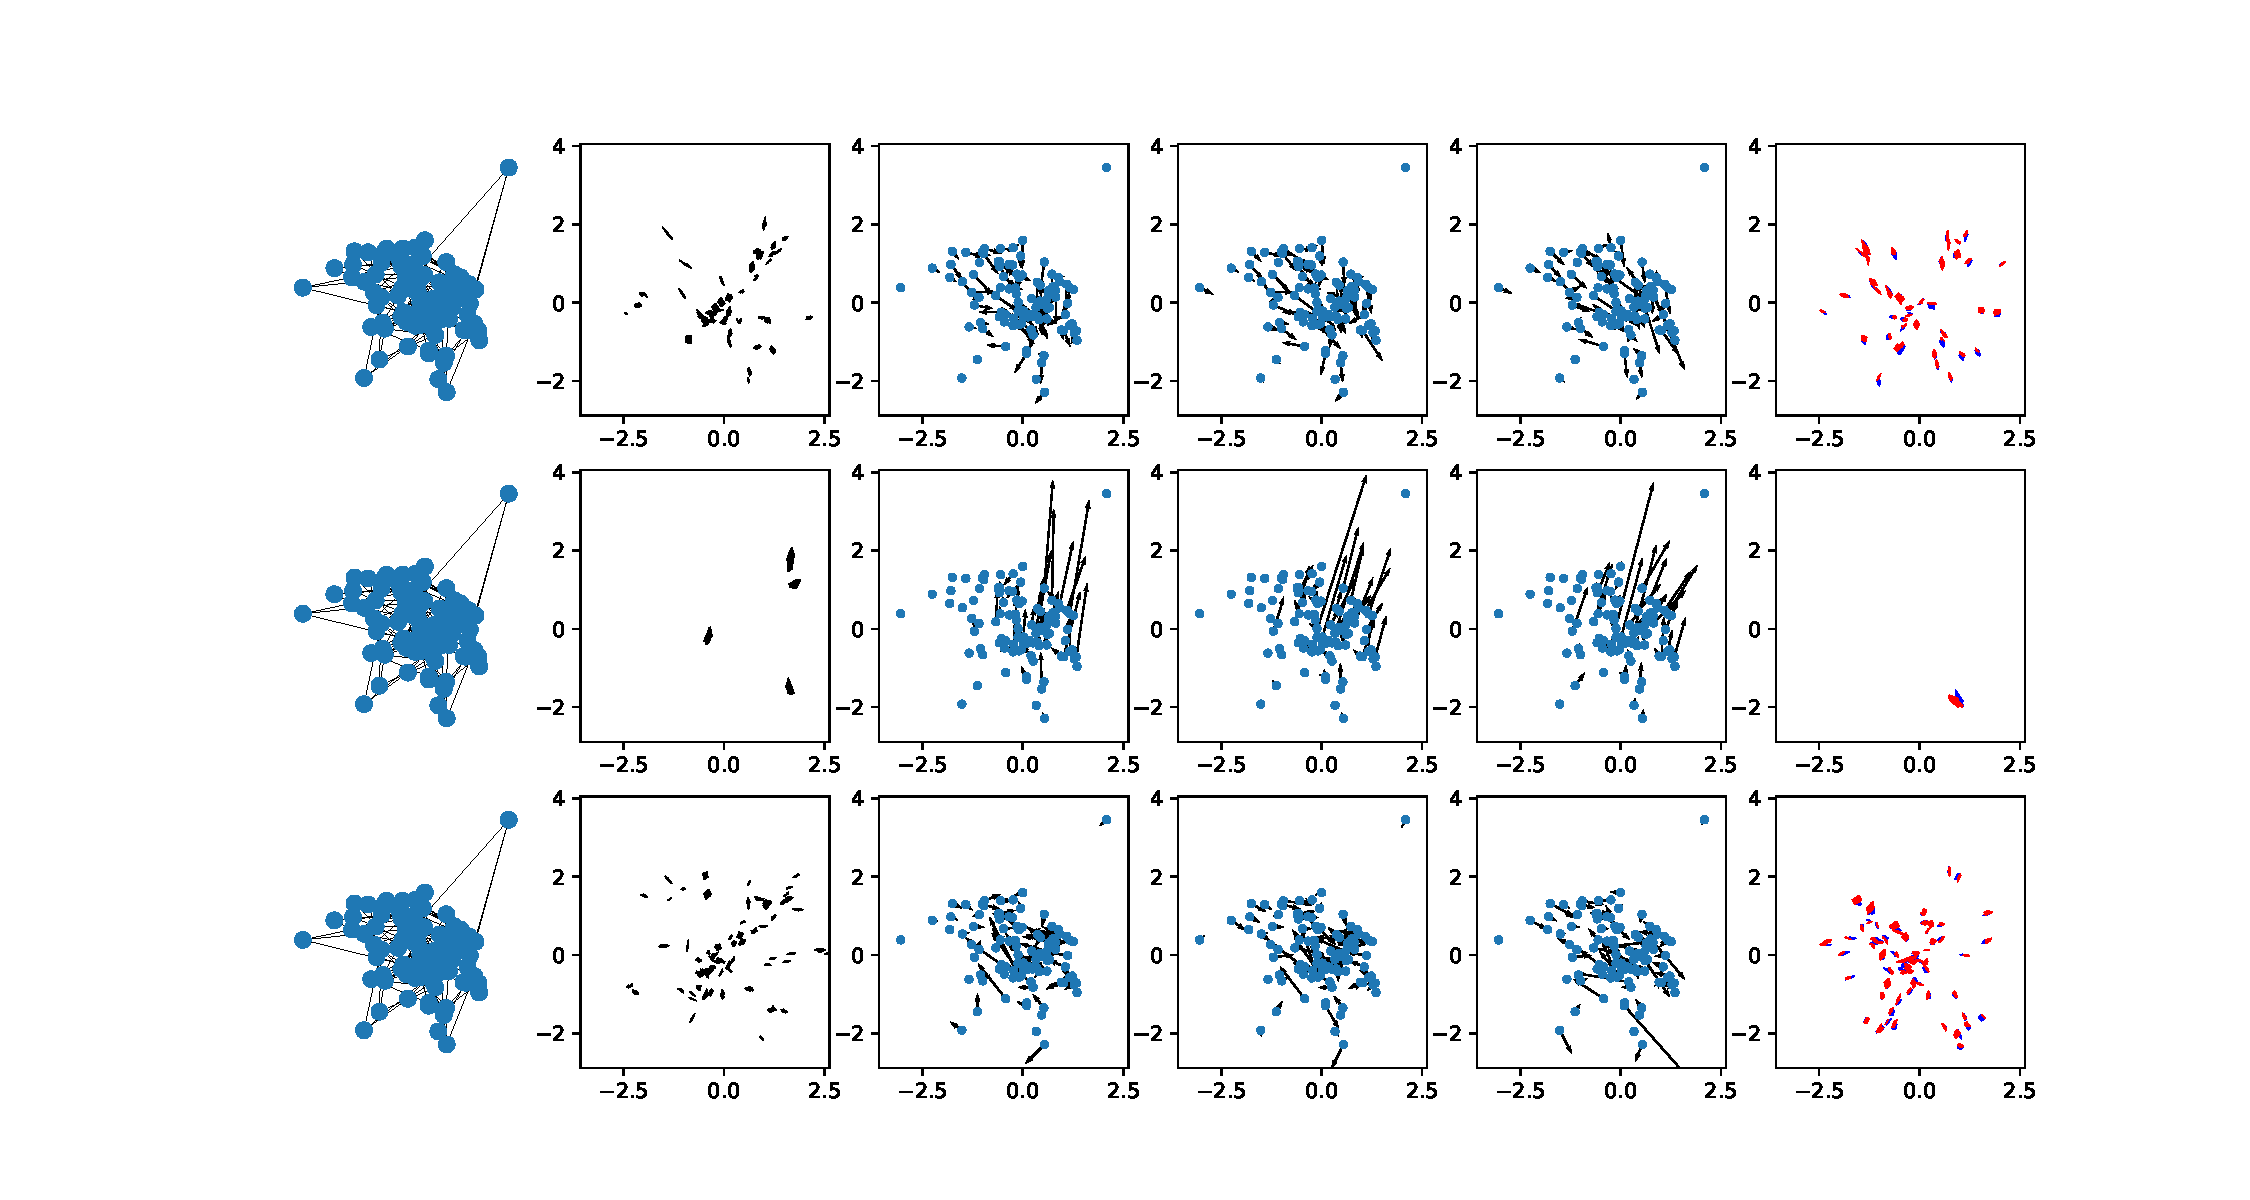
\includegraphics[trim={0 13.2cm 29cm 0},clip,width=\textwidth]{../results/pdfs/nn-100N-noemb0}
    \caption{$k$-means, 3nn}
  \end{subfigure}
  \begin{subfigure}{0.24\textwidth}
    \centering
    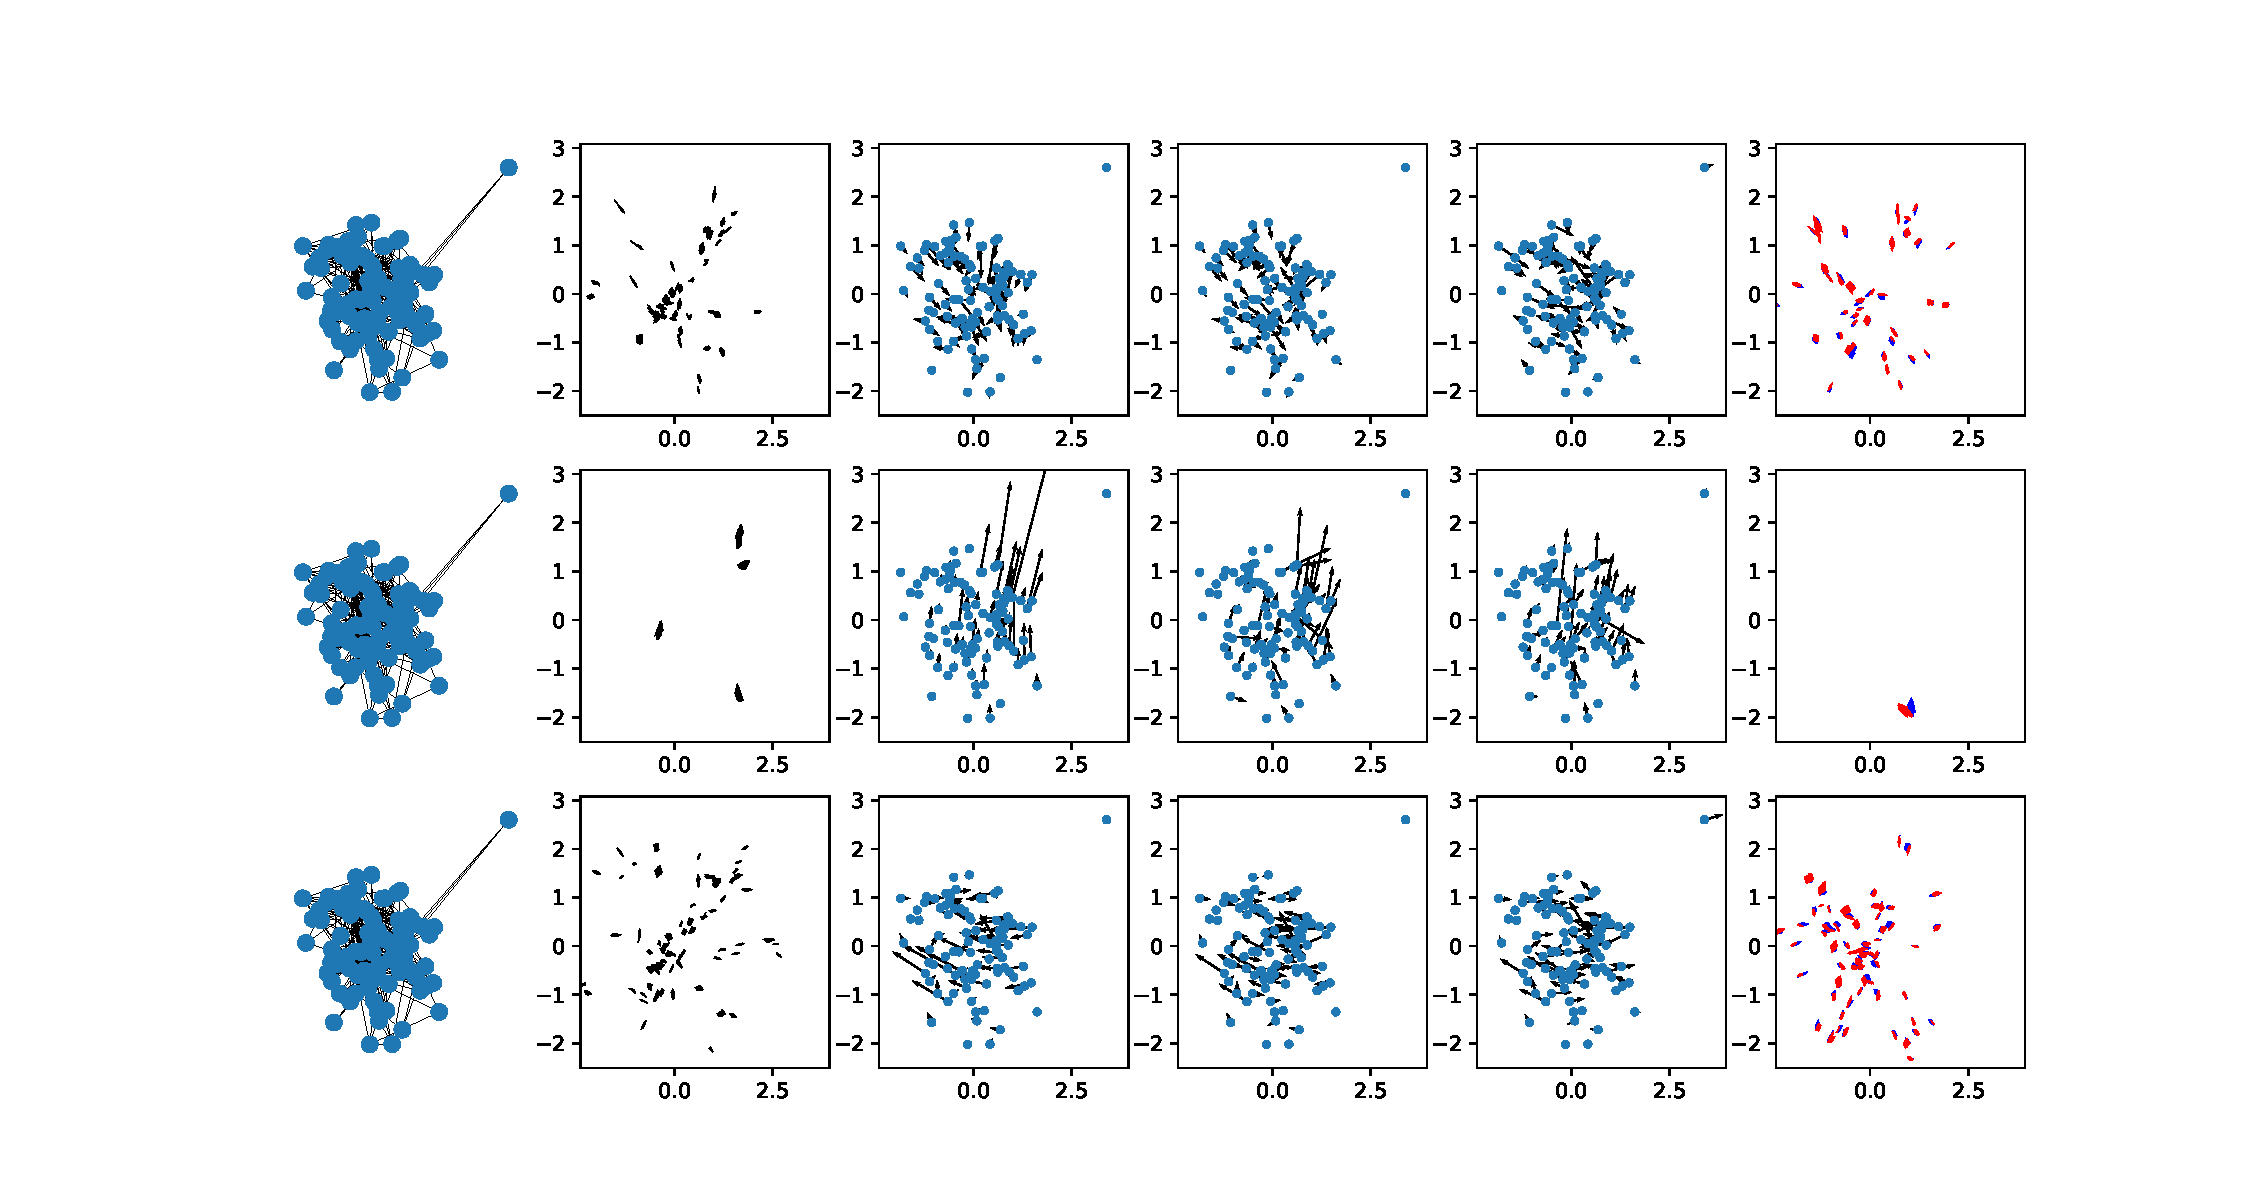
\includegraphics[trim={0 13.2cm 29cm 0},clip,width=\textwidth]{../results/pdfs/ba-100N-noemb0}
    \caption{$k$-means, BA}
  \end{subfigure}
  \caption{Graph structure for the different models. The first row (a-d) show graphs where each node has a fixed position, in the second row (e-h) we see how this position has evolved during training.}
  \label{fig:graphs}
\end{figure}

\begin{table*}
  \centering
  \begin{tabular}{lcccc} \toprule
    \multirow{2}{*}{\textbf{Model}}                      &                            & \multicolumn{3}{c}{\textbf{Nodes}}                                                           \\ \cmidrule(lr){3-5}
                                                         &                            & 10                                 & 100                    & 1000                           \\ \hline
    \multirow{2}{*}{\textbf{Random Network, $p=1\%$} }   & \scriptsize \textsc{Fixed} & 0.80  \tiny $\pm$ 0.04             & 0.71  \tiny $\pm$ 0.02 & 0.70 \tiny $\pm$ 0.02          \\
                                                         & \scriptsize \textsc{Adapt} & 0.69 \tiny $\pm$ 0.01              & 0.65 \tiny $\pm$ 0.02  & \textbf{0.64 \tiny $\pm$ 0.02} \\
    \multirow{2}{*}{\textbf{Random Network, $p=10\%$}}   & \scriptsize \textsc{Fixed} & 0.76  \tiny $\pm$ 0.03             & 0.70  \tiny $\pm$ 0.02 & 0.76 \tiny $\pm$ 0.02          \\
                                                         & \scriptsize \textsc{Adapt} & 0.69 \tiny $\pm$ 0.01              & 0.66 \tiny $\pm$ 0.01  & 0.66 \tiny $\pm$ 0.02          \\
    \multirow{2}{*}{\textbf{$k$-means, 3 nn.}          } & \scriptsize \textsc{Fixed} & 0.68  \tiny $\pm$ 0.01             & 0.69  \tiny $\pm$ 0.02 & 0.68 \tiny $\pm$ 0.01          \\
                                                         & \scriptsize \textsc{Adapt} & 0.68 \tiny $\pm$ 0.01              & 0.66 \tiny $\pm$ 0.01  & 0.65 \tiny $\pm$ 0.01          \\
    \multirow{2}{*}{\textbf{$k$-means, BA}             } & \scriptsize \textsc{Fixed} & 0.69  \tiny $\pm$ 0.01             & 0.68  \tiny $\pm$ 0.01 & 0.66 \tiny $\pm$ 0.02          \\
                                                         & \scriptsize \textsc{Adapt} & 0.68 \tiny $\pm$ 0.02              & 0.65 \tiny $\pm$ 0.02  & \textbf{0.64 \tiny $\pm$ 0.01} \\

    \bottomrule
  \end{tabular}
  \caption{
    We tried different graph topologies for our model that use no embeddings. First, as a baseline, we tried Random Networks, where the position of each node is drawn from $\mathcal{U}(-1,1)$ and where there is an edge between two nodes with probability $p$. Then we tried to use $k$-means to get the position of the nodes and added edges either between the 3 nearest neighbors in the graph or following a Barabasi-Albert procedure. The results are the MSE error on the validation set, we ran ten different seeds to get the standard deviation. All measures are normalized.
  }
  \label{tab:graphs}
\end{table*}


\subsection{Nodes and Edge features}

\begin{table*}
  \label{tab:nodes}
  \centering
  \begin{tabular}{lcccc} \toprule
    \multirow{2}{*}{\textbf{Model}}                     &                            & \multicolumn{3}{c}{\textbf{Nodes}}                                                          \\ \cmidrule(lr){3-5}
                                                        &                            & 10                                 & 100                            & 1000                  \\ \hline
    \multirow{2}{*}{\textbf{No Emb}}                    & \scriptsize \textsc{Fixed} & 0.68 \tiny $\pm$ 0.01              & 0.69 \tiny $\pm$ 0.02          & 0.68 \tiny $\pm$ 0.01 \\
                                                        & \scriptsize \textsc{Adapt} & 0.68 \tiny $\pm$ 0.01              & 0.66 \tiny $\pm$ 0.01          & 0.65 \tiny $\pm$ 0.01 \\
    \multirow{2}{*}{\textbf{MLP}}                       & \scriptsize \textsc{Fixed} & 0.66 \tiny $\pm$ 0.01              & 0.66 \tiny $\pm$ 0.02          & 0.67 \tiny $\pm$ 0.02 \\
                                                        & \scriptsize \textsc{Adapt} & 0.66 \tiny $\pm$ 0.01              & 0.64 \tiny $\pm$ 0.01          & 0.64 \tiny $\pm$ 0.03 \\
    \multirow{2}{*}{\textbf{Added Pos-Enc,MLP}}         & \scriptsize \textsc{Fixed} & 1.03 \tiny $\pm$ 0.04              & 1.06 \tiny $\pm$ 0.02          & 1.04 \tiny $\pm$ 0.02 \\
                                                        & \scriptsize \textsc{Adapt} & 1.07 \tiny $\pm$ 0.07              & 1.04 \tiny $\pm$ 0.03          & 1.03 \tiny $\pm$ 0.02 \\
    \multirow{2}{*}{\textbf{Concat Pos-Enc,MLP}}        & \scriptsize \textsc{Fixed} & 0.65 \tiny $\pm$ 0.01              & 0.63 \tiny $\pm$ 0.01          & 0.65 \tiny $\pm$ 0.02 \\
                                                        & \scriptsize \textsc{Adapt} & 0.65 \tiny $\pm$ 0.02              & \textbf{0.63 \tiny $\pm$ 0.01} & 0.64 \tiny $\pm$ 0.01 \\
    \multirow{2}{*}{\textbf{Concat Pos-Enc,MLP,Edges }} & \scriptsize \textsc{Fixed} & 0.XX \tiny $\pm$ 0.XX              & 0.XX \tiny $\pm$ 0.XX          & 0.XX \tiny $\pm$ 0.XX \\
                                                        & \scriptsize \textsc{Adapt} & 0.XX \tiny $\pm$ 0.XX              & \textbf{0.XX \tiny $\pm$ 0.XX} & 0.XX \tiny $\pm$ 0.XX \\

    \bottomrule
  \end{tabular}
  \caption{
    We tried different types of node embeddings for our model. The first one is the baseline is to use no embedding layer and keep the aggregated wind value as the node state. The second one uses a small MLP encoder to project the wind value to a higher-dimensional space. Finally, we explored two versions of the positional encoding layer. The results are the MSE error on the validation set, we ran ten different seeds to get the standard deviation. All measures are normalized.
  }
\end{table*}

We tried four different ways of embeddings the information in the nodes. The results of the different experiments can be found in Table \ref{tab:nodes}. We ran ten experiments, changing the seed, for each node embedding and the position of the graph could be optimized in the case where the structure is fixed. We first use no embeddings at all, using directly the measurements values. This allowed us to see the processing performed by the network [Fig.\ref{fig:processing}]. We found that using no embeddings and delegating all the processing to the message passing layers was already performing on par with the best models. We think that the models are powerful enough to process the information and that the other approach needs to learn an additional encoding/decoding network which might require longer training to reach the best accuracy. We trained all the models for 10 epochs (but each epoch contains roughly 33 M measurements) so in that range, the simpler model might be easier to learn. The best performing embedding was using an MLP on top of concatenated positional encodings. This might help the model process the information at a different scale and apparently, it helps a little. Finally, we found that adding the positional encodings altogether was decreasing a lot the accuracy of the model. Maybe under this representation distinguishing between positions is harder for the model.

\subsection{Edge Features}
We added edge features to the graph, that encode the distance between the nodes or the finite difference between the initial node features.

\begin{figure}[htbp]
  \centering
  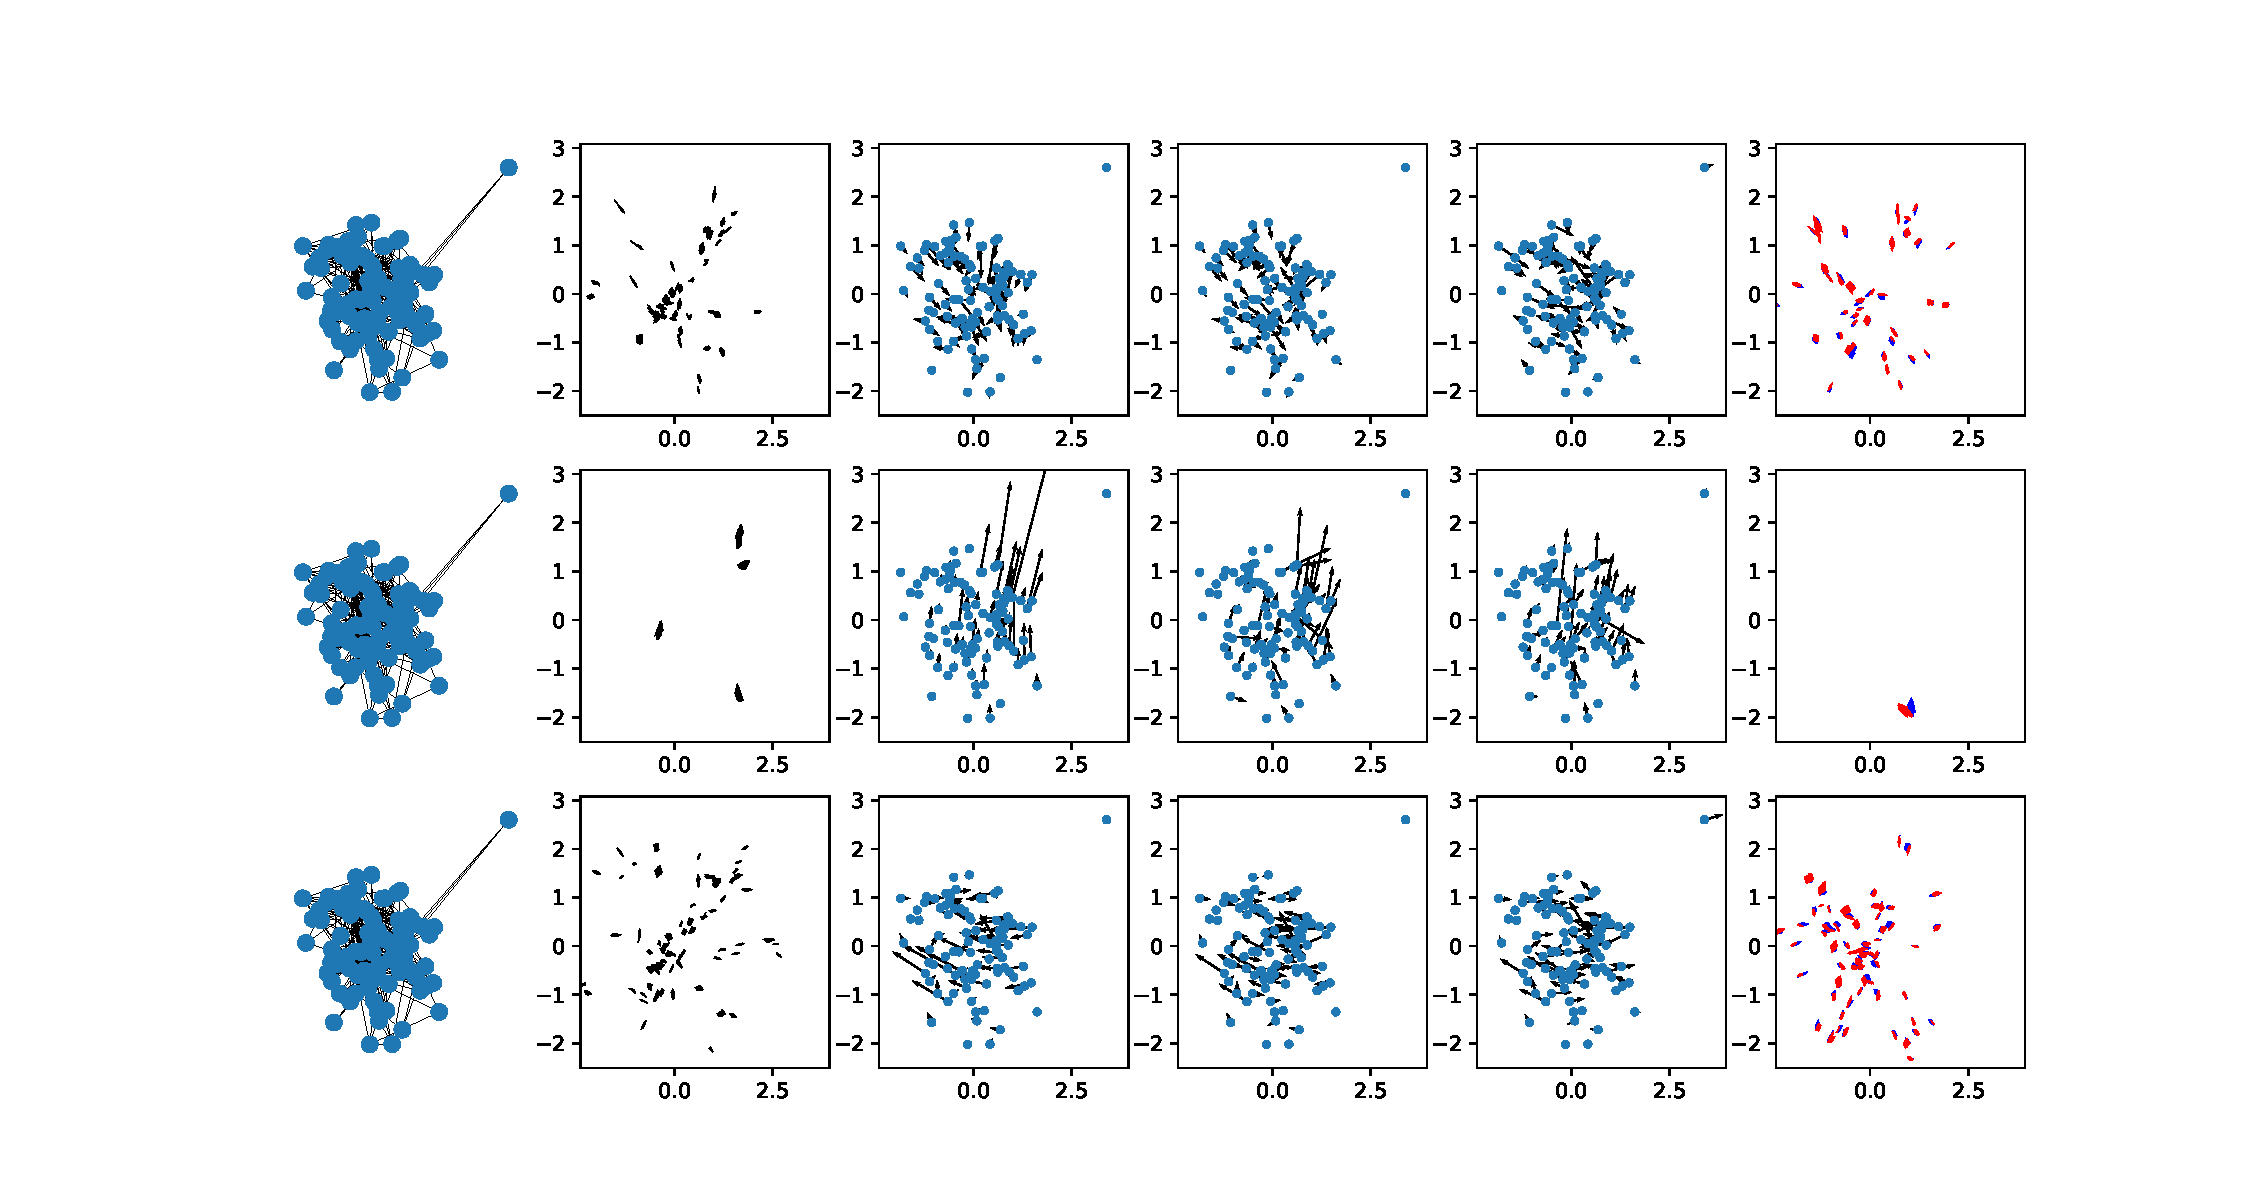
\includegraphics[width=\textwidth]{../results/pdfs/ba-100N-noemb0.pdf}
  \caption{Using no-embeddings allows to visualize the model processing the info layer after layer. The first column shows the graph structure, the second represents a minibatch of data that is then encoded (third column), then we see two steps of message passing and the decoded values.}
  \label{fig:processing}
\end{figure}



\section{Conclusion}
We used graph networks to forecast the wind speed at cruising altitudes on a horizon of 30min. Graph Networks were able to efficiently process measurements sparsely distributed in the space. This architecture has a good inductive bias for this problem as each node is capable of approximating a part of the space. As the dataset at our disposal is sparse with most of the measurements clustered along some main routes, graph networks are more efficient than other grid-based solvers such as traditional PDEs solvers or CNN. We started by reimplementing the architecture presented in \cite{alet2019gen}. We used several graph structures and different node embeddings. We found that using graphs with hubs and edges between far-away nodes helps the model process the information efficiently. We found that the model doesn't need to have special embeddings as the message-passing architecture is powerful enough, but adding a small MLP encoder with concatenated positional encodings helps a bit.


\bibliographystyle{apalike}
\bibliography{main}
\section{Appendix}
\FloatBarrier
\begin{table*}
  \centering
  \begin{tabular}{llrr} \toprule
                                        &                   & \textbf{Arnaud}    & \textbf{Yasmin} \\ \midrule
    \multirow{4}{*}{\textbf{Homeworks}} & HW1               & 100 \%             &                 \\
                                        & HW2               & 1-version + review &                 \\
                                        & HW3               & 100 \%             &                 \\
                                        & HW4               & 100 \%             &                 \\ \cmidrule{2-4}
    \multirow{3}{*}{\textbf{Project}}   & Code              & 100 \%             &                 \\
                                        & Report            & 100 \%             &                 \\
                                        & Slides            &                    &                 \\
                                        & Presentation tool &                    &                 \\
    \bottomrule
  \end{tabular}
  \caption{ Workload repartition between the two teammates \color{red} TODO : Yasmin write your contributions here}
  \label{tab:nodes}
\end{table*}


\end{document}